%%%%%%%%%% !TEX program = pdflatex %%%%%%%%%%
% !TEX program = pdflatex
\documentclass[a4paper,12pt,openany,twoside]{book}

% 当目录多于1页时,使用\thispagestyle{empty}和\pagestyle{empty},都无法完全清除目录的页眉页脚格式,需要使用到下面的\AtBeginDocument{}代码
\AtBeginDocument{
	\addtocontents{toc}{\protect\thispagestyle{empty}}%
	\addtocontents{lof}{\protect\thispagestyle{empty}}%
}

                                           % 如果论文超过60页 可以使用twoside 双面打印
% !TEX program = pdflatex
% !Mode:: "TeX:UTF-8"
%  Authors: 杜家宜   Jiayi Du: Max_dujiayi@gmail.com     湖南大学2010级计算机科学与技术专业博士生

%%%%%%%%%% Package %%%%%%%%%%%%
\usepackage[chapter]{algorithm}
\usepackage{pdfpages}% 方便插入签字版权页
%\usepackage{algorithmic}
\usepackage{etoolbox}
\usepackage{algpseudocode}

\usepackage{graphicx}                       % 支持插图处理
\usepackage{geometry}
\geometry{left=2.5cm,right=2.5cm,top=2cm,bottom=2.5cm,footskip=1.1cm,headsep=0.7cm,head=0.4cm}
% 支持版面尺寸设置
\usepackage{titlesec}                       % 控制标题的宏包
\usepackage{titletoc}                       % 控制目录的宏包
\usepackage{fancyhdr}                       % fancyhdr宏包 支持页眉和页脚的相关定义
\usepackage[UTF8]{ctex}                    % 支持中文显示
\usepackage{cite}
\usepackage{color}                          % 支持彩色
\usepackage{amsmath}                        % AMSLaTeX宏包 用来排出更加漂亮的公式
\usepackage{amssymb}                        % 数学符号生成命令
\usepackage{mathrsfs}                       % Add by Lijianmin
\usepackage{cases}
\usepackage[below]{placeins}                %允许上一个section的浮动图形出现在下一个section的开始部分,还提供\FloatBarrier命令,使所有未处理的浮动图形立即被处理
\usepackage{flafter}                        % 使得所有浮动体不能被放置在其浮动环境之前,以免浮动体在引述它的文本之前出现.
\usepackage{multirow}                       % 使用Multirow宏包,使得表格可以合并多个row格
\usepackage{colortbl}						% 表格颜色
\usepackage{booktabs}                       % 表格,横的粗线;\specialrule{1pt}{0pt}{0pt}
\usepackage{longtable}                      % 支持跨页的表格。
\usepackage{tabularx}                       % 自动设置表格的列宽
\usepackage{setspace}
\usepackage{subfigure}                      % 支持子图 %centerlast 设置最后一行是否居中
\usepackage[subfigure]{ccaption}            % 支持子图的中文标题
\usepackage{booktabs}                       % 用于绘制三线表

%\usepackage{hologo}
%\usepackage[super]{gbt7714}

\usepackage[sort&compress,numbers]{natbib}  % 支持引用缩写的宏包
\usepackage{enumitem}                       % 使用enumitem宏包,改变列表项的格式
\usepackage{calc}                           % 长度可以用+ - * / 进行计算
\usepackage{txfonts}                        % 字体宏包
\usepackage{bm}                             % 处理数学公式中的黑斜体的宏包
\usepackage[amsmath,thmmarks,hyperref]{ntheorem}  % 定理类环境宏包,其中 amsmath 选项用来兼容 AMS LaTeX 的宏包
\usepackage{CJKnumb}                        % 提供将阿拉伯数字转换成中文数字的命令
\usepackage{indentfirst}                    % 首行缩进宏包
\usepackage{CJKutf8}                        % 用在UTF8编码环境下,它可以自动调用CJK,同时针对UTF8编码作了设置。
\usepackage{CJK}
\usepackage{fancyhdr}
\usepackage{lastpage}
\usepackage{layout}
\usepackage[titles,subfigure]{tocloft}      %控制生成的表格和图片的目录格式
%\usepackage{caption}
% Add by Lijianmin
%\usepackage{hypbmsec}                      % 用来控制书签中标题显示内容
%\usepackage{bbding}
%如果您的pdf制作中文书签有乱码使用如下命令,就可以解决了
%Modified by Lijianmin
\usepackage[unicode,               % pdflatex, pdftex 这里决定运行文件的方式不同
%\usepackage[dvipdfm, unicode,               % pdflatex, pdftex 这里决定运行文件的方式不同
pdfstartview=FitH,
%CJKbookmarks=true,
bookmarksnumbered=true,
bookmarksopen=true,
colorlinks=true,
pdfborder={0 0 1},
citecolor=black,
linkcolor=black,
anchorcolor=black,
urlcolor=black,
breaklinks=true
]{hyperref}
                      % 定义本文所使用宏包
\graphicspath{{figures/}}                  % 定义所有的.eps文件在figures子目录下
\begin{document}                           % 开始全文
\begin{CJK*}{UTF8}{song}                   % 开始中文字体使用
\input{setup/format}                       % 完成对论文各个部分格式的设置

\frontmatter                               % 以下是论文导言部分,包括论文的封面,中英文摘要和中文目录

\clearpage
% !Mode:: "TeX:UTF-8"

%%% 封面填写部分 

\classnumber{TP37}
\schoolcode{10590}
\UDCnumber{UDCnumber}
\security{公开}

\cheading{深圳大学硕士学位论文}
\thesisTitle{RISC-V高性能处理器分支预测部件研究} %封面用论文标题,自己可手动断行
\cdegree{工程硕士专业学位}
\college{计算机与软件学院} %学院名称
\majorName{计算机技术}   %专业
\authorName{邹\space江\space瑞}   %学生姓名
\supervisor{蔡晔} %导师姓名

% 使用makecover生成封面
\makecover							% 封面

% % !Mode:: "TeX:UTF-8"

%%%% 原创性声明填写部分 %%%

\declaretitle{原创性声明}
\declarecontent{
	本人郑重声明: 所呈交的学位论文\underline{基于RISC-V高性能处理器的分支预测部件研究}是本人在导师的指导下,独立进行研究工作所取得的成果。除文中已经注明引用的内容外,本论文不含任何其他个人或集体已经发表或撰写过的作品或成果。对本文的研究做出重要贡献的个人和集体,均已在文中以明确方式标明。本声明的法律结果由本人承担。
}
\authorizationtitle{学位论文版权使用授权书}
\authorizationcontent{
	本学位论文作者完全了解深圳大学关于收集、保存、使用学位论文的规定,即:研究生在校攻读学位期间论文工作的知识产权单位属深圳大学。学校有权保留学位论文并向国家主管部门或其他机构送交论文的电子版和纸质版,允许论文被查阅和借阅。本人授权深圳大学可以将学位论文的全部或部分内容编入有关数据库进行检索,可以采用影印、缩印或扫描等复制手段保存、汇编学位论文。
}
\authorizationadd{(涉密学位论文在解密后适用本授权书)}
\authorsigncap{作者签名:}
\supervisorsigncap{导师签名:}
\signdatecap{签字日期:}

% 使用makecopyright生成原创性说明
\makecopyright 与 \includepdf{data/copyright.pdf} 二选一
%% !Mode:: "TeX:UTF-8"

%%%% 原创性声明填写部分 %%%

\declaretitle{原创性声明}
\declarecontent{
	本人郑重声明: 所呈交的学位论文\underline{基于RISC-V高性能处理器的分支预测部件研究}是本人在导师的指导下,独立进行研究工作所取得的成果。除文中已经注明引用的内容外,本论文不含任何其他个人或集体已经发表或撰写过的作品或成果。对本文的研究做出重要贡献的个人和集体,均已在文中以明确方式标明。本声明的法律结果由本人承担。
}
\authorizationtitle{学位论文版权使用授权书}
\authorizationcontent{
	本学位论文作者完全了解深圳大学关于收集、保存、使用学位论文的规定,即:研究生在校攻读学位期间论文工作的知识产权单位属深圳大学。学校有权保留学位论文并向国家主管部门或其他机构送交论文的电子版和纸质版,允许论文被查阅和借阅。本人授权深圳大学可以将学位论文的全部或部分内容编入有关数据库进行检索,可以采用影印、缩印或扫描等复制手段保存、汇编学位论文。
}
\authorizationadd{(涉密学位论文在解密后适用本授权书)}
\authorsigncap{作者签名:}
\supervisorsigncap{导师签名:}
\signdatecap{签字日期:}

% 使用makecopyright生成原创性说明
\makecopyright                        % 诚信说明
\includepdf{data/copyright.pdf}             % 使用pdf文件替换原有的诚信声明data/copyright

% !Mode:: "TeX:UTF-8"

%%% 中文摘要填写部分 %%%

\cabstract{

    在现代的高性能处理器设计领域中,分支预测是一个处理器架构中必不可少的一部分,处理器为了追求更高的性能往往会往高频率,深流水线的方向设计,高频率就限制了每周期内逻辑的复杂度,而深流水线则会使分支预测错误带来的惩罚更高。关于分支预测算法的研究有很多,还有CBP (Championship Branch Prediction) 这样的分支预测赛事促进分支预测发展,TAGE预测器是目前公开设计的先进分支预测器之一,曾多次获得CBP比赛的冠军。但是分支预测研究的论文大多基于模拟器实现,而真实的硬件设计过程中会有更多的约束和细节需要考虑。
    本文基于香山RISC-V开源高性能处理器第一版架构的基础上,设计了第二版分支预测架构,旨在实现解耦前端的设计以达到更高的性能,同时通过减少分支预测宽度来减关键路径的延迟,达到更高的频率。另外还尝试了一些分支预测相关的优化和探索。首先我们通过添加一个FTQ (Fetch Target Queue) 来讲分支预测与取指逻辑解耦,通过FTQ来保存分支预测结果,控制分支预测恢复和更新。此外,通过改进BTB (Branch Target Buffer),我们将取指的基本单位由第一版的32Bytes对齐的定长指令块改为了以fetch block为单位的不定长指令块,以此来限制每次取指的分支指令数量,并将所有预测器的基本单位也都修改为使用fetch block预测。
    通过使用Verilator进行行为级仿真,并使用checkpoint技术来运行SPEC 2006的片段来评估整体架构性能,通过性能计数器来统计(具体的性能提升数据)
    综上所述,本文研究了RISC-V高性能处理器的分支预测架构,以及物理实现过程中的具体问题,提出并完成了一种分支预测的具体实现。最终通过行为级仿真对齐进行了评估,实验结果表明相对于第一版架构,新的设计有xxx的提升。

}

\ckeywords{RISC-V;~~高性能处理器;~~CPU设计;~~解耦前端;~~分支预测}

\cnpageheader{摘要}  %页眉标题无需断行

% 使用makecnabstract生成中文摘要
\makecnabstract						% 中文摘要
% !Mode:: "TeX:UTF-8"

%%% 英文摘要填写部分 %%%

\enabstract{

    In the field of modern high-performance processor design, the Branch Prediction Unit (BPU) is an essential part of a processor architecture, in order to pursue higher performance, processors are often designed in the direction of high frequency and deep pipeline, High frequency limits the complexity of logic per cycle, and deep pipelines incur higher penalties for branch misprediction. There is a lot of research on branch prediction algorithms. For example, the TAGE predictor is one of the state-of-the-art branch predictors currently publicly designed. However, most of the papers on branch prediction research are based on simulator implementation, and there are more constraints and physical implementation details to be considered in the real hardware design process.

    Based on the first version of the Yanqihu architecture of Xiangshan RISC-V open source high-performance processor, this thesis designs the Branch Prediction Unit in the second version of the Nanhu architecture. The Nanhu architecture is a new architecture that is reconstructed and upgraded on the Yanqihu architecture.Because the Branch Prediction Unit contains multiple critical paths of the Yanqihu architecture, and in the test, it is found that the frontend fetch bubbles account for a large proportion of the overall running cycle. Therefore, the main challenge faced by the Branch Prediction Unit of the Nanhu architecture is how to reduce the fetch bubbles and achieve a higher frequency on the premise of ensuring the accuracy of the original Branch Prediction Unit.The new Branch Prediction Unit is designed to decouple the Branch Prediction Unit and the Instruction Fetch Units for higher performance, while reducing critical path latency by reducing the branch prediction width for higher frequencies. The following is the main research content of this thesis:

    (1) By improving BTB (Branch Target Buffer), the basic unit of instruction fetch is changed from the 32 Bytes-aligned fixed-length instruction block of Yanqihu architecture to the variable-length instruction block with Fetch Block as the unit, this limits the maximum number of branch instructions per fetch, and also modified all predictors to use Fetch Block as base prediction unit.

    (2) The Branch Prediction Unit is decoupled from the Instruction Fetch Unit by adding an FTQ (Fetch Target Queue), which is used to save instruction fetch requests and branch prediction results, and control branch prediction recovery and update.

    The main innovation of this thesis is to propose and implement a branch prediction architecture suitable for decoupling the frontend, and a branch prediction architecture that limits the width of branch prediction, which can bring both performance and frequency improvements to the processor. It is the first implementation in the field of RISC-V open source processor research. 

    Evaluate overall architecture performance by performing behavioral-level simulations with Verilator, and using checkpointing techniques to run snippets of SPEC CPU 2006, with performance counters for statistics and analysis. Compared with the first version. 

    In summary, this thesis studies the branch prediction architecture of RISC-V high-performance processors, as well as the specific problems in the physical implementation process, and proposes and completes a specific implementation of branch prediction. Finally, it is evaluated by behavioral simulation. The experimental results show that compared with the Yanqihu architecture, the frequency of Nanhu can be increased 11\% under the 14nm process, and the IPC of some SPEC CPU 2006 test programs is increased by an average of 31\%. 

}

\enkeywords{RISC-V;~~high performance processor;~~CPU;~~decoupled frontend;~~branch prediction}

\enpageheader{Research on Branch Prediction Component Based on RISC-V High Performance Processor}

% 使用makeenabstract生成英文摘要
\makeenabstract						% 英文摘要

\clearpage
\pagestyle{empty}		% modified by Jon: 去掉页眉页脚
% 目录
\renewcommand{\contentsname}{\erhao\song\bfseries\hspace*{\fill}目\quad 录\hspace*{\fill}}    % 设置“目录”二字的格式
\tableofcontents                           % 中文目录

\clearpage
\cleardoublepage

% 正文部分
\defaultfont
\pagestyle{plain}
\mainmatter\sloppy\raggedbottom
%\renewcommand{\ALC@linenosize}{\xiaosi}
\renewcommand\arraystretch{1.5}
\setlength{\intextsep}{2pt}
\setlength{\abovecaptionskip}{2pt}
\setlength{\belowcaptionskip}{2pt}

% 内容比较多的时候,编译速度较慢,可以将不同章节放在不同文件中,注释掉其他章节,只编译正在撰写的章节,以提升编译速度
% !Mode:: "TeX:UTF-8"

\chapter{绪论}

\section{研究背景及意义}
CPU (Central Processing Unit) 是一台计算机最重要最核心的组成部分,也叫做中央处理器。在现代生活中,各种各样的服务器,电脑,手机,小型电子设备无处不在,已经成为了现代人生活的重要组成部分。CPU属于处理器的一种,同样是处理器,也能分为很多不同的类型,如图\ref{fig:figure14}所示,有用于服务器上的,执行大量复杂计算任务的高性能处理器,也有用于手机、路由器、蓝牙设备等对功耗有一定要求的低功耗芯片,用于图像渲染的GPU,专门针对深度学习,人工智能相关的计算进行了特定优化的AI处理器等等。处理器设计制造也一直是高精尖的技术领域。这部分的先进技术大部分掌握在美国手中。自2020年美国开始禁止向中国出口高端芯片以来,使得芯片成为了这两年的热点话题,也给国内的芯片行业敲响了警钟,我国更加注重处理器设计领域的发展,推出了一系列相关政策推动我国加快发展自己的芯片设计和制造产业。国内的多家企业和高校也都积极响应,开始重视自主可控的芯片设计开发以及相关技术人才的培养。例如龙芯杯和一生一芯计划\cite{ysyx},都旨在为我国培养高端的芯片设计人才。以龙芯为首的多家国内企业多年以来也一直不断地在相关领域内投入研发,到目前为止也有了不俗的成果。虽然还没能完全摆脱对国外芯片的依赖,但是国内芯片产业已经有逐渐崛起的趋势。

\begin{figure}[htb]
    \centering
    \setlength\tabcolsep{3pt}  % 同一行中的图片间隔
    \vspace{5pt} % 图片上部的空白,如果太小的话,图片顶部会与正文内容十分接近
    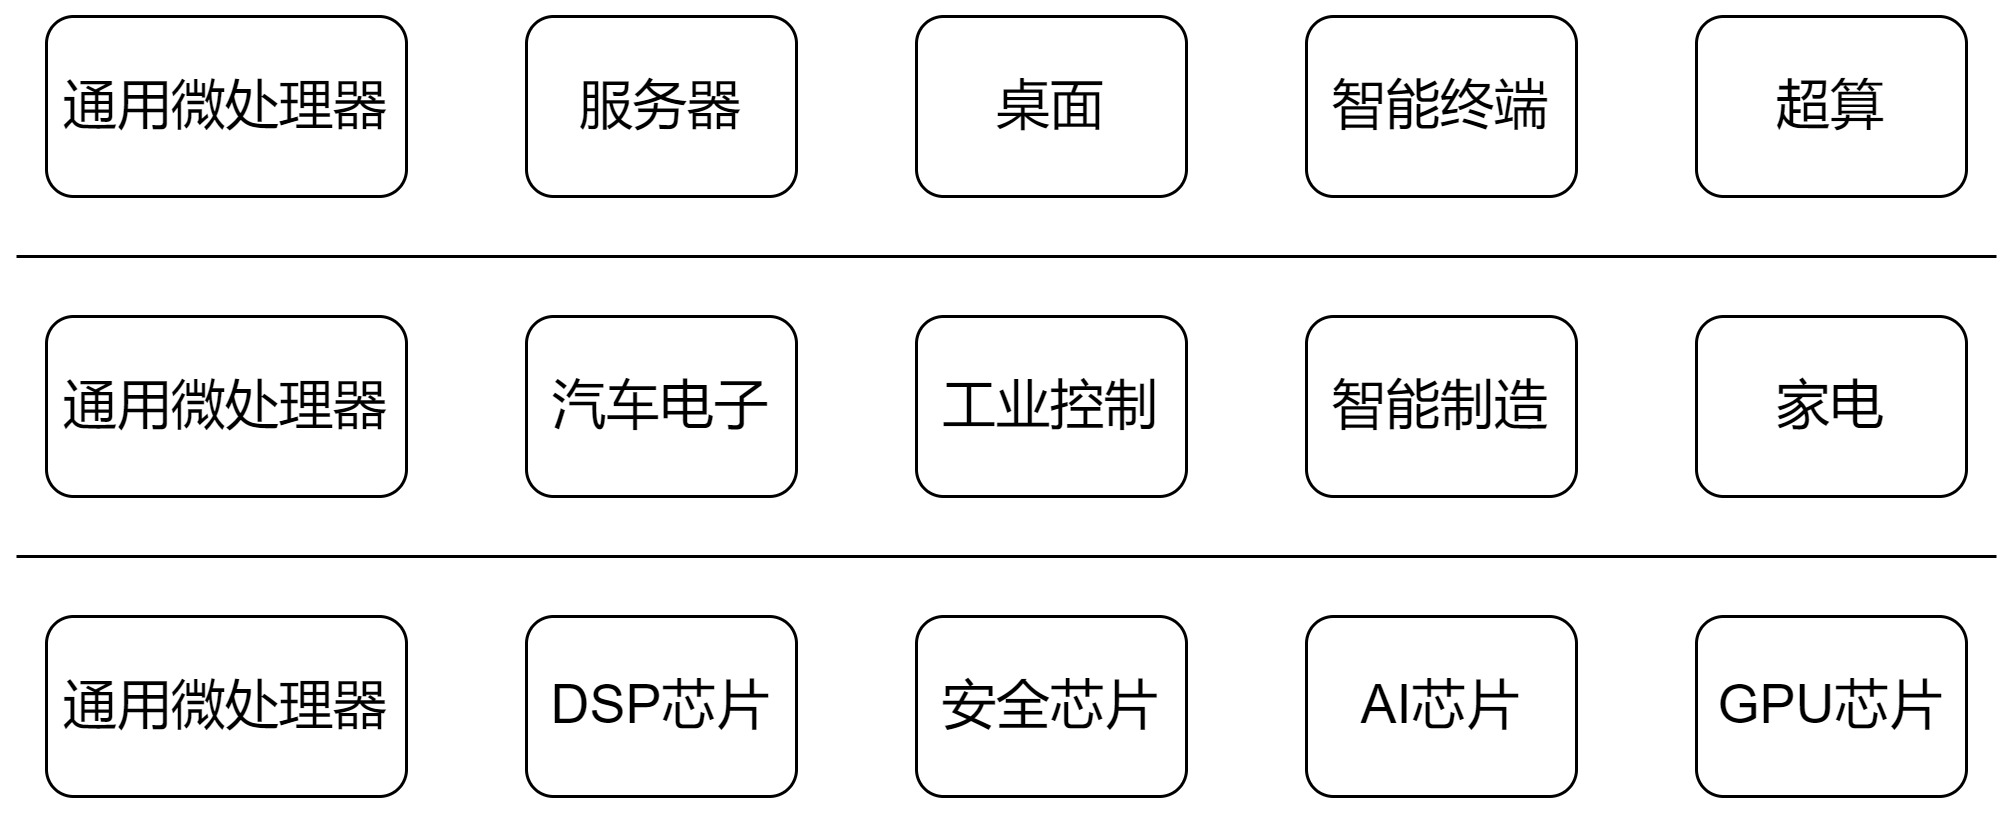
\includegraphics[width=1\textwidth]{processor-cate.jpg}
    \caption{不同领域的处理器分类\cite{cpu-overview}}
    \label{fig:figure14}
\end{figure}

如图\ref{fig:figure13}所示目前市场上的处理器可以按照指令集类型分为两大类:CISC (复杂指令集) 和RISC (精简指令集) \cite{cpu-overview},市面大多使用的是x86和ARM指令集架构,分别对应了CISC和RISC两大类,其中x86的指令集架构掌握在Intel手中,x86架构的处理器主要是Intel和AMD这两家美国公司占主流,主打产品是一些高性能计算机的处理器。基本上所有的服务器和电脑上搭载的都是这些公司的CPU。处于高性能领域的垄断地位。ARM指令集架构掌握在ARM公司手中,而ARM公司主要靠指令架构的授权来盈利,而不自己设计制造芯片。ARM架构的处理器广泛的使用在各种嵌入式产品和终端中,在现在万物互联的趋势下普及到生活的各个角落中。这两个架构几乎垄断了各类高端处理器的市场,如果有一家企业想要设计制造一款处理器,无法避免的需要到x86或者ARM的指令集授权,支付一笔昂贵的费用,极大提高了芯片的成本。这样会极大的阻碍其他企业想要设计开发芯片的热情,也会影响整个产业的创新与进步。在这种局面下,急需一个更加友好开放的新鲜血液注入到市场中,才能为整个产业带来新的活力。

\begin{figure}[htb]
    \centering
    \setlength\tabcolsep{3pt}  % 同一行中的图片间隔
    \vspace{5pt} % 图片上部的空白,如果太小的话,图片顶部会与正文内容十分接近
    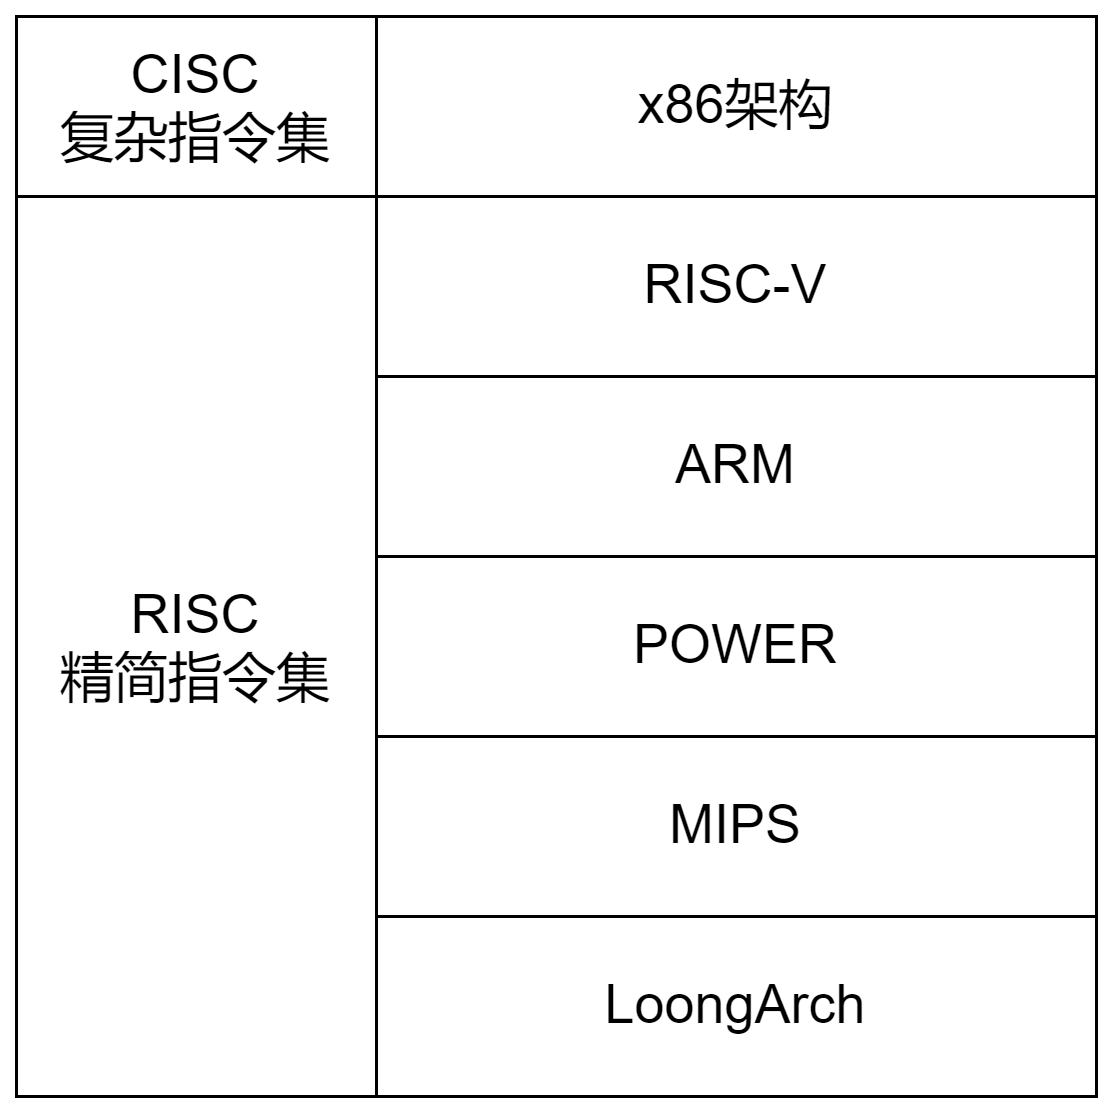
\includegraphics[width=0.5\textwidth]{isa.png}
    \caption{指令集架构分类}
    \label{fig:figure13}
\end{figure}

而RISC-V的出现打破了这一局面,RISC-V是2010年始于美国加州大学伯克利分校的一款开源指令集架构\cite{riscv-overview},与大多数指令集相比,RISC-V指令集没有高昂的授权费用,任何人都可以使用RISC-V设计和制造芯片,而不用支付任何费用。这极大的降低了芯片的成本。同时由于这是一个年轻的指令集架构,没有x86和ARM由于需要兼容老旧的设计而带来的历史包袱,例如现代的处理器基本都是64位,而x86和ARM为了兼容以前的老机器,在设计时还需要考虑在32位机器上的兼容性问题。RISC-V使用了更先进的模块化设计理念。因此RISC-V一经面世,就受到了业内的关注和支持,尤其是在受到美国制裁的前提下,RISC-V非常适合我国的国情,我国的许多企业都加入了RISC-V基金会,在RISC-V基金会的19位高级成员中,有11位都是中国企业,比例已经超过半数。

% \begin{figure}[htb]
% 	\centering
% 	\setlength\tabcolsep{3pt}  % 同一行中的图片间隔
% 	\vspace{5pt} % 图片上部的空白,如果太小的话,图片顶部会与正文内容十分接近
% 	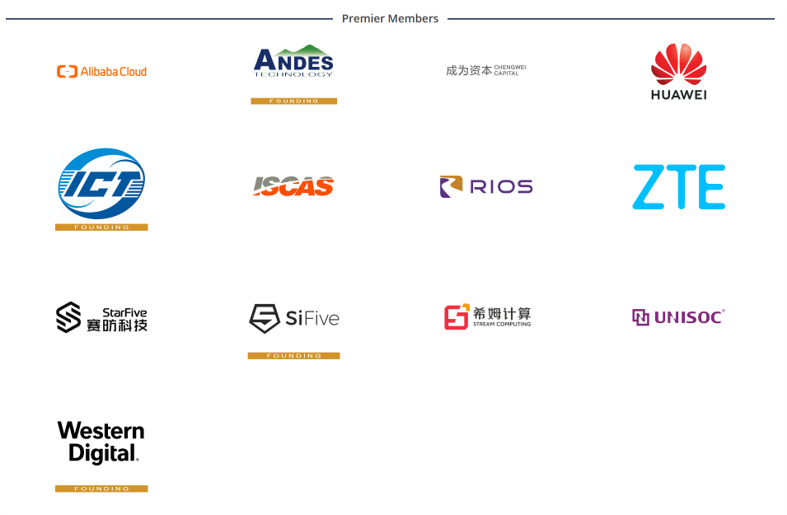
\includegraphics[width=1\textwidth]{RISC-V_Foundation_Members.png}
% 	\caption{RISC-V 基金会高级成员(评委老师说这张图要删掉)}
% 	\label{fig:figure1}
% \end{figure}

早期的RISC-V由于还在逐渐发展,大家对其仍然抱着观望的态度,主要还是用在一些功能比较简单的嵌入式芯片设计中,使用RISC-V设计的高性能处理器仍然较少,甚至早期还有人说RSIC-V不能用于开发高性能处理器。但是近几年来不断有国内的企业开始使用RISC-V设计高性能处理器,例如阿里巴巴的玄铁系列\cite{xuantie},而中科院计算所也研发了一款开源的RISC-V高性能处理器,命名为香山\cite{xiangshan},希望能够通过开源香山以及香山的开发流程和工具,探索高校设计制造处理器的可行性,并且希望能够搭建出一整套完善的集开发、调试、评估为一体的迭代流程。以此带动各路开发者的热情,打造一个良好的社区,促进处理器相关领域的发展。希望大家能够积极的参与到香山的开发与完善,也希望有人能够以香山为平台进行计算机体系结构的研究,未来更希望能有企业使用香山芯片制造出自己的产品。而本文的研究就是在香山处理器的开发平台上进行的。香山的第一版架构设计被命名为雁栖湖,在雁栖湖架构的基础上,对处理器中所有的模块进行了大量的改进和升级,实现了香山第二版架构,命名为南湖。目前香山雁栖湖架构版本已经流片成功,南湖架构版本已经完成了时序调优,后端测试无误后即将送往流片。

在一个高性能处理器架构里,分支预测是必不可少的一个部件。由于分支指令会导致处理器的指令流水线出现中断,因此一个高效的分支预测部件能够尽可能地减少流水线中断的情况,极大提升处理器的整体性能,同时也能够降低流水线执行无效指令产生的额外功耗。由于现代的处理器都在往更高的频率,更深的流水线发展,以期待获得更高的性能。但同时更高的频率也限制了每个流水级间逻辑门级的数量,更深的流水线则造成了更大的分支误预测惩罚。并且处理器执行的程序指令数量也变得越来越多。在这种前提下,导致分支预测性能即使是一点点小小的提升,都能够对处理器的整体性能带来不可忽视的改变。因此高性能处理器的不断发展对分支预测的设计带来了更大的挑战\cite{bpu-overview},如何在满足频率要求的前提下实现预测算法,并且保证较高的分支预测准确率,是所有工程师和学者们都不断在研究推进的课题,各种各样的预测算法不断被提出,改进。

香山处理器雁栖湖架构的分支预测参考了加州大学伯克利分校开发的一款开源RISC-V处理器BOOM (The Berkeley Out-of-Order Machine) 的分支预测设计\cite{boom-spec}。该分支预测设计有4级流水,使用混合预测器,以TAGE预测器作为主要的预测器。之所以选择以BOOM作为参考,首先是由于它作为一款开源的高性能处理器,可以直接接触到源代码,方便学习理解,且BOOM有过一次成功流片的经验,在业内的认可度也比较高。其次由于设计代码与香山开发使用的是相同的Chisel语言\cite{chisel},因此BOOM能够为香山带来许多的参考思路。例如香山在开发中有借鉴BOOM的参数管理机制,以及一些使用了Chisel语言特性的设计。

在讨论先进的分支预测算法和设计时,现有的论文大多基于模拟器来建模研究,没有考虑到具体的硬件实现,以及针对高频的优化。在真实的物理设计中,由于硬件特性和时序要求,相对于论文中的设计,在某些地方可能需要做出针对性的修改和优化,才能够将其真正的在硬件上实现。除了BOOM以外,有先进分支预测架构的开源设计也是寥寥无几,只能够通过公司的相关产品介绍和论文中窥到一些细节。因此本文以国内开源RISC-V高性能处理器香山为研究平台,在雁栖湖架构的基础上对分支预测进行了重构和优化,使其能够达到更高的性能和频率,最终应用到雁栖湖架构的下一代升级版本南湖架构中。同时,所有的设计代码都是开源的,能够给RISC-V社区中的开发者们提供借鉴和启发。

\section{国内外研究现状}


\subsection{RISC-V发展现状}
RISC-V是加州大学伯克利分校在2010年首次发布的一个开源指令集架构,2015年成立RISC-V基金会,而国内在2018年也成立了中国RISC-V产业联盟 (CRVIC)。这是一个年轻的指令集架构,它是吸收了大量已有指令集,如x86,ARM,MIPS等指令集的设计经验,弥补了它们的不足,做出大量的改进后产生的,并且为了给体系结构领域注入新的活力,RISC-V拥抱开源,使用RISC-V无需支付任何费用,让全世界的开发者能够不受成本政治等边缘因素的影响,全新的投入到RISC-V的设计与开发中来。

除了开源免费以外,RISC-V作为一个全新的指令集架构,不需要考虑历史兼容性的问题,这也使得它能够更加精简,门槛更低,相比于x86和ARM动辄几千页的手册,RISC-V的手册只有寥寥几百页,学习门槛大大降低,开发者们能够在更短的时间内掌握RISC-V设计的基础。并且RISC-V考虑到针对不同领域的不同需求,使用了模块化设计,除了基本的几十条指令以外,其他的都被模块化为一个个的扩展,开发者可以根据具体应用的需要,实现不同的扩展,而不用将所有的指令都实现,这使得RISC-V非常的多变与灵活,开发者也可以在RISC-V的基础上实现自定义指令,来满足产品的功能需求。

由于多种因素,RISC-V一出世就受到了工业界和学术界的关注与肯定。在经过一段时间的发展与完善后,大家都开始尝试以RISC-V为基础进行研究与设计。大量的研究成果也不断发布,最具代表性的就是加州大学伯克利分校的Rocket\cite{rocket}和BOOM两款开源的处理器设计,其中BOOM作为开源高性能处理器的代表,更是在大量的论文中作为研究平台和对比对象。而国内也有大量的成果,例如在阿里巴巴2021年9月10日正式开源的玄铁910,就是一款使用RISC-V指令集的处理器。此外国内还有很多公司都有相关的产品,如华米科技的黄山1号、紫光展锐的春藤系列,以及兆易创新的GD32VF103等。随着越来越多企业的加入,RISC-V也在不断地完善和发展自己的生态,

\subsection{分支预测发展现状}

分支预测器也有着不同的类型,首先是最简单的静态分支预测,静态分支预测通过一些静态的信息来进行预测,而不会考虑指令动态执行时的不同情况,例如可以将所有的分支都预测为跳转或不跳转\cite{branch-98},或者将向后跳转的分支预测为跳转,将向前的分支预测为不跳转。与之对应的就是更复杂,更准确的动态分支预测。动态分支预测能够通过收集程序运行时指令的动态信息来进行训练,学习到分支指令跳转的模式,根据不同情况给出预测,这样能够达到更加高的准确率,当然同时就对预测算法与硬件实现提出了更高的要求。由于更高的预测准确率,因此大部分处理器还是使用动态预测器为主。也有一些预测器不作为主要的预测器,而是作为在某个特定场景下使用的辅助预测器,比如循环预测器用于学习嵌套循环中循环指令的迭代次数,还有返回地址栈 (Return Address Stack, RAS),专门用于预测函数调用和返回指令的跳转地址。包括还有一些使用神经网络或机器学习来训练程序,以达到更高的分支预测准确率的研究\cite{branch-neural,branch-not-resolved,fast-neural-branch}。

分支预测器按照功能也分为两类,一种是方向预测器,比如TAGE预测器,这类预测器在预测时只会给出指令是否跳转的预测,而不会给出指令的跳转地址。另一种就是地址预测器,比如间接跳转预测器,用于在预测间接跳转分支时给出跳转地址。最常见的地址预测器就是各种各样的BTB (Branch Target Buffer)了,用于在还没有得到指令预译码信息时给出分支指令的跳转地址,并且有着许多不同的设计和实现。

此外分支预测器也可以按照使用的分支历史分为局部历史预测器和全局历史预测器。程序执行时可以记录所有分支指令的跳转历史,用1表示跳转,0表示不跳转,通过这些历史对预测器进行训练,找到特定的模式来为后续的分支指令做预测。局部历史预测器倾向于使用部分的分支历史来做预测,例如循环预测器只会寻找可能是循环跳转指令的分支。而全局历史预测器会倾向于使用所有的分支历史或某种全局分支历史的哈希,例如TAGE预测器。两种类型的预测器都各有优劣,因此将它们混合使用往往可以更好的覆盖不同的分支指令。

在现在的主流高性能处理器中一般使用的都是混合分支预测器,即同时包含多种预测器,在不同的情况下分别选择使用不同预测器的预测结果,以达到覆盖更多类型分支,以及满足硬件设计要求的目的。通常会有一个简单的预测器,它的预测速度很快,一个周期就能够给出预测结果,用于保证分支预测流水线不会中断,然后还有一个主要的预测器,可能需要2-3个周期才会出预测结果,包括还有很多使用机器学习和神经网络来训练分支预测来达到更高的分支预测准确率的研究。最终会根据不同情况,选择最合适的预测器的预测结果送往取指。

\subsection{现有处理器的分支预测设计}

\begin{itemize}[listparindent=2em]
	\item BOOM (the Berkeley Out-
    of-Order Machine)\cite{boom-spec, sonic-boom}使用了耦合的前端设计,总共有4级取指流水级,其中在F1,F2,F3会分别得到不同预测器的预测结果,并且当后面的预测结果和前面不同时,需要纠正前面的错误预测。在F1使用Micro BTB进行预测,F2使用BIM和BTB进行预测,F3使用TAGE进行预测。
    
    此外BOOM还实现了循环预测器和RAS (Return Address Stack),循环预测器用于在某些嵌套循环指令中,预测循环体的循环跳转指令。RAS用于预测call和return指令。

    \begin{figure}[htb]
        \centering
        \setlength\tabcolsep{3pt}  % 同一行中的图片间隔
        \vspace{5pt} % 图片上部的空白,如果太小的话,图片顶部会与正文内容十分接近
        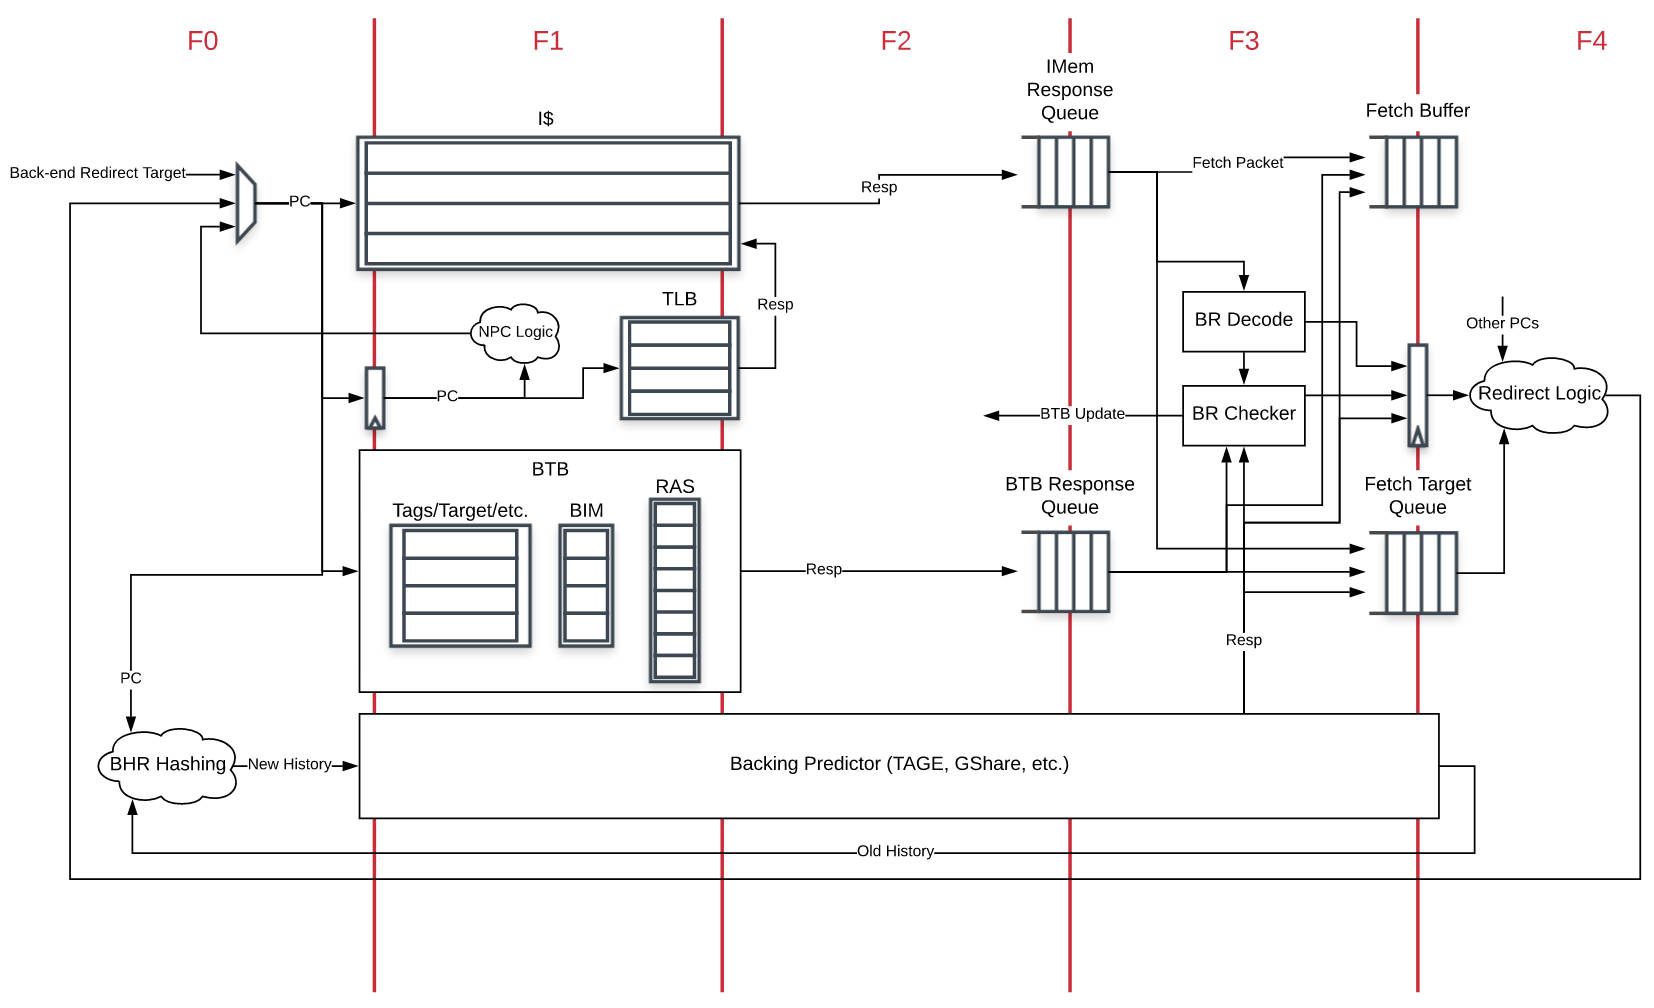
\includegraphics[width=1\textwidth]{boom-frontend.jpg}
        \caption{BOOM前端架构图\cite{boom-frontend}}
        \label{fig:figure11}
    \end{figure}

	\item 玄铁910\cite{xuantie}使用了耦合的前端设计,即取指单元和分支预测流水级是耦合的,采用了两级的混合预测器的结构设计。在IP级就可以得到预译码信息,可以直接解析出一些直接跳转指令的跳转目标地址。

    玄铁910使用BHT(branch target table)来存储分支跳转历史,使用了一种类似BI-MODE\cite{bi-mode}机制的方向预测器。在IF级有一个16项全相联的L0 BTB (Branch Target Buffer),在IP级有一个1K项组相联的L1 BTB。使用覆盖预测,当IP级的预测结果与IF级不同时需要将之前的预测结果纠正回来。这种设计和香山雁栖湖架构是类似的。

    此外玄铁910还有支持12级函数调用嵌套的RAS;循环加速器 (Loop Buffer),用于将循环体中的指令缓存下来,关闭指令缓存来节省功耗;间接跳转预测器,用于预测间接跳转指令的目标地址。

    \item 龙芯GS464E\cite{loongson}前端依然是耦合的设计,总共有3个流水级,也是多种预测器混合使用,在每周期最多可以处理4条分支指令。龙芯GS464E中实现了一个分支目标缓冲器 (BrBTB),功能类似于BOOM的Micro BTB,都是为了在更准确的预测器结果出来之前,做一个简单的预测,尽可能提高流水线的连续性,不同之处在于龙芯GS464E的BrBTB是放在IF4级流水级的。除了BrBTB外,还有更加准确的预测器,实现了一套组合分支历史表 (BHTs),包含3张16K项的表,分别是全局转移历史表 (global branch history table, GBHT),局部转移历史表 (local branch history table, LBHT)和全局选择历史表 (global branch select table, GSEL)。此外还有RAS,和用于预测间接跳转指令的跳转目标缓存器 (jump branch target address cache, JBTAC),和玄铁910类似的Loop Buffer。
    
    
    \begin{figure}[htb]
        \centering
        \setlength\tabcolsep{3pt}  % 同一行中的图片间隔
        \vspace{5pt} % 图片上部的空白,如果太小的话,图片顶部会与正文内容十分接近
        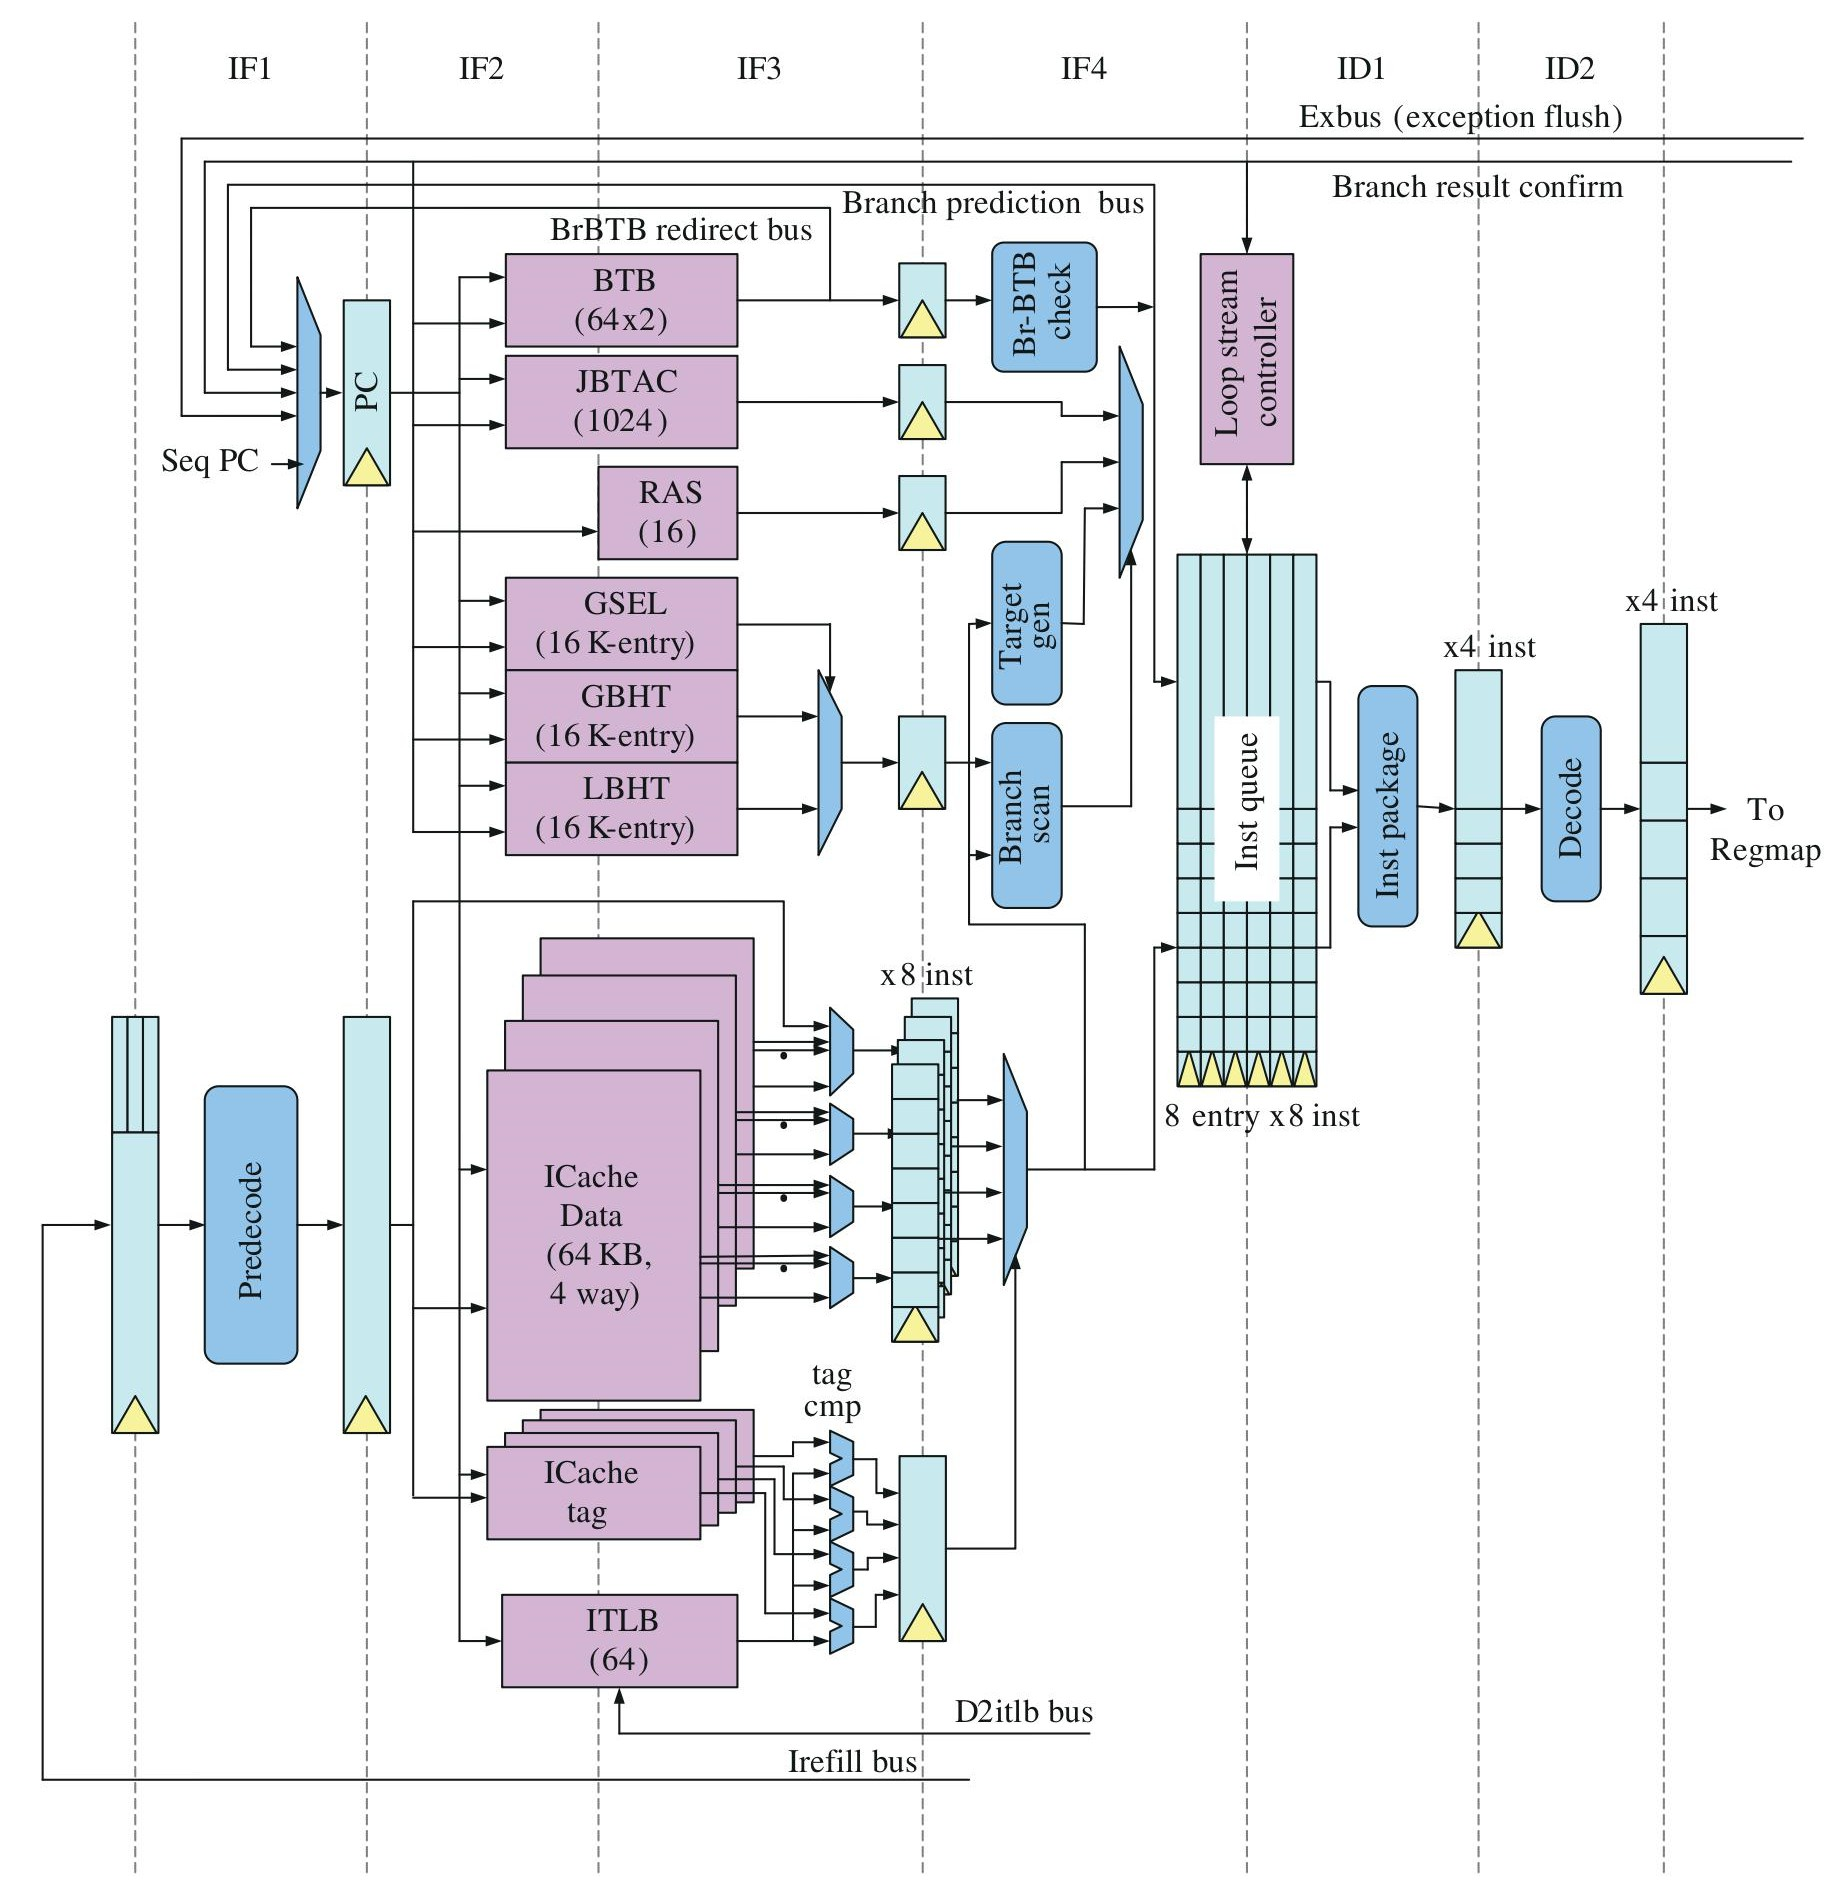
\includegraphics[width=1\textwidth]{loongson-frontend.jpg}
        \caption{龙芯GS464E前端架构图\cite{loongson}}
        \label{fig:figure12}
    \end{figure}
    
    \item Samsung Exynos\cite{samsung-exynos}使用了解耦的前端,主要的分支预测器使用的是改进的Scaled Hashed Perceptron (SHP)算法\cite{perceptrons,neural-branch,optimized-neural,strided-perceptron,merging-perceptron,revisited-perceptron},同样是混合预测,有一个小而快的micro-BTB (μBTB) 和一个本地历史散列感知器 (LHP),主要的分支预测器是main-BTB (mBTB)和SHP。还实现了RAS,Level-2 BTB (L2BTB) 以及virtual address-based BTB (vBTB)。间接跳转预测器使用的是virtual program counter (VPC)\cite{vpc} 预测器。
\end{itemize}

从以上几个处理器的分支预测设计可以看出,目前混合预测的设计是主流方案,一般倾向于一个小而快的预测器搭配上一个准但是慢的主要预测器,再加上一些针对特定指令的预测器,例如RAS和间接跳转预测器等。虽然在以上几个处理器设计中只有Samsung Exynos是解耦前端,但是根据与其他设计团队的交流来看,解耦前端确实是目前主流商用处理器都在使用的一个方案。

% \subsection{引用参考文献}
% 在references.bib中添加参考文献对应的bibtex,使用$\backslash$cite\{\}引用论文的id,如引用参考文献\cite{barnes2009patchmatch}。

% \subsection{插入图片}
% 如图\ref{fig:figure1}所示,在文章中插入图片。使用$\backslash$begin\{figure\}插入图片,支持的格式有jpg、png、eps与pdf等,本例使用$\backslash$begin\{tabular\}插入三幅图像(一行三列),如果只插入一副图像则不需使用$\backslash$begin\{tabular\}。

% \begin{figure}[htb]
% 	\centering
% 	\setlength\tabcolsep{3pt}  % 同一行中的图片间隔
% 	\vspace{5pt} % 图片上部的空白,如果太小的话,图片顶部会与正文内容十分接近
% 	\begin{tabular}{ccc}
% 		\includegraphics[width=0.32\textwidth]{baboon.jpg} &
% 		\includegraphics[width=0.32\textwidth]{lena.jpg} &
% 		\includegraphics[width=0.32\textwidth]{parrot.jpg} \\
% 		(a) 图1 & (b) 图2 & (c) 图3 \\[1ex]
% 	\end{tabular}
% 	\caption{图片示例}
% 	\label{fig:figure1}
% \end{figure}

% \subsection{插入公式}
% 如公式\eqref{eq:equation1}所示,为公式示例:
% \begin{equation}
% 	c = a + b
% 	\label{eq:equation1}
% \end{equation}

% \subsection{插入表格}

% 如表格\ref{tb:table1}所示,为表格示例。可以通过"https://www.tablesgenerator.com/"以用户界面形式创建表格,并将表格转化为latex代码。

% \begin{table}[]
% 	\caption{表格标题}
% 	\label{tb:table1}
% 	\centering
% 	\begin{tabular}{|c|c|c|}
% 		\hline
% 		a   & b   & c   \\ \hline
% 		1.1 & 1.2 & 1.3 \\ \hline
% 		1.4 & 1.5 & 1.6 \\ \hline
% 	\end{tabular}
% \end{table}

\section{本文思路及研究方法}

本文首先介绍了开源RISC-V高性能处理器在国内的研究意义,以及为什么选择使用RISC-V来设计处理器的原因,然后简单介绍了分支预测的发展现状,不同类型的预测器以及它们各自的特点。之后介绍了本课题的研究平台,即由中科院研发的开源处理器香山,对香山超标量乱序处理器分支预测的基本结构和各个预测器的功能和设计思路做了介绍。进一步介绍了分支预测部件的整体架构,并在此基础上从性能和频率两个方面对其进行了优化。

\begin{itemize}
	\item 性能方面。通过将雁栖湖架构的前端分支预测和取指部分解耦,减少了前端流水线由于分支预测和取指单元共用流水级导致的不必要的阻塞。其中主要介绍了FTQ (Fetch Target Queue)这个主要模块的功能和行为逻辑。
	\item 频率方面。为了减少分支预测整体的预测宽度,将整个分支预测的基本单位由单条分支改为了Fetch Block,通过定义约束来限制每次取指的block中分支指令的上限。主要介绍FTB (Fetch Target Buffer)这个主要模块的功能和行为逻辑。
\end{itemize}

介绍完相关的优化之后,我们使用Design Compiler对整个处理器架构进行了时序评估,并使用Verilator对整体设计进行行为级仿真,运行SPEC2006测试程序,通过分析相关的性能数据用于评估其改进结果。

\section{论文结构}

本文分为以下几个章节,内容安排如下:

第一章的主要内容是介绍了本课题的研究背景和意义,讨论了一些国内外的研究现状,分支预测器的分类。简单介绍了香山处理器的整体架构,并对本文内容做了规划。

第二章的主要内容是介绍分支预测架构流水级,以及各个流水级中预测器的分布,然后介绍各个预测器的功能及其设计实现细节。

第三章的主要内容是介绍以FTB为主的限制分支预测宽度的分支预测改进策略,并给出了FTB的详细数据结构设计,以及更新管理策略。

第四章的主要内容是提出以FTQ为主的实现解耦前端取指单元的设计,详细介绍了FTQ与分支预测、取指单元、后端执行单元交互的各种功能和逻辑。

% 第五章的主要内容是介绍了针对改进分支预测性能做过的部分尝试及其细节

第五章的主要内容是介绍开发和评估测试设计所用到的环境,以及相关的评估指标,统计结果及其分析。

第六章的主要内容是对本文工作的一个总结,并指出目前仍然存在的一些问题,提出了一些已知的改进方向,对之后的工作做出了展望。

 							
% !Mode:: "TeX:UTF-8"
\chapter{分支预测器介绍}


本章首先介绍香山处理器第二版分支预测的整体架构,各个预测器在流水级中的先后关系和联系。其次针对每个预测器都介绍了它们的预测原理和功能。并指出它们相对于第一版设计做出的修改,以及做出相关修改的原因。

\section{分支预测整体结构}

香山第二版分支预测架构采用的是4级流水设计,架构图如图\ref{fig:figure21}所示。参考了BOOM提出的COBRA架构\cite{cobra},能够更加灵活的管理和组织预测器。在4个流水级中,S0主要负责收集S1、S2、S3流水级的预测结果,以及取指单元 (Instruction Fetch Unit, IFU)和流水线后端 (Backend) 发回的分支误预测信息,从中选择出下一周期需要进行预测的指令pc (Program Countet),即指令在其内存中的地址。然后将该pc以及其他用于预测的信息发给各个预测器,不同的预测器得出预测结果的时间需要1到2周期不等。

\begin{figure}[htb]
	\centering
	\setlength\tabcolsep{3pt}  % 同一行中的图片间隔
	\vspace{5pt} % 图片上部的空白,如果太小的话,图片顶部会与正文内容十分接近
	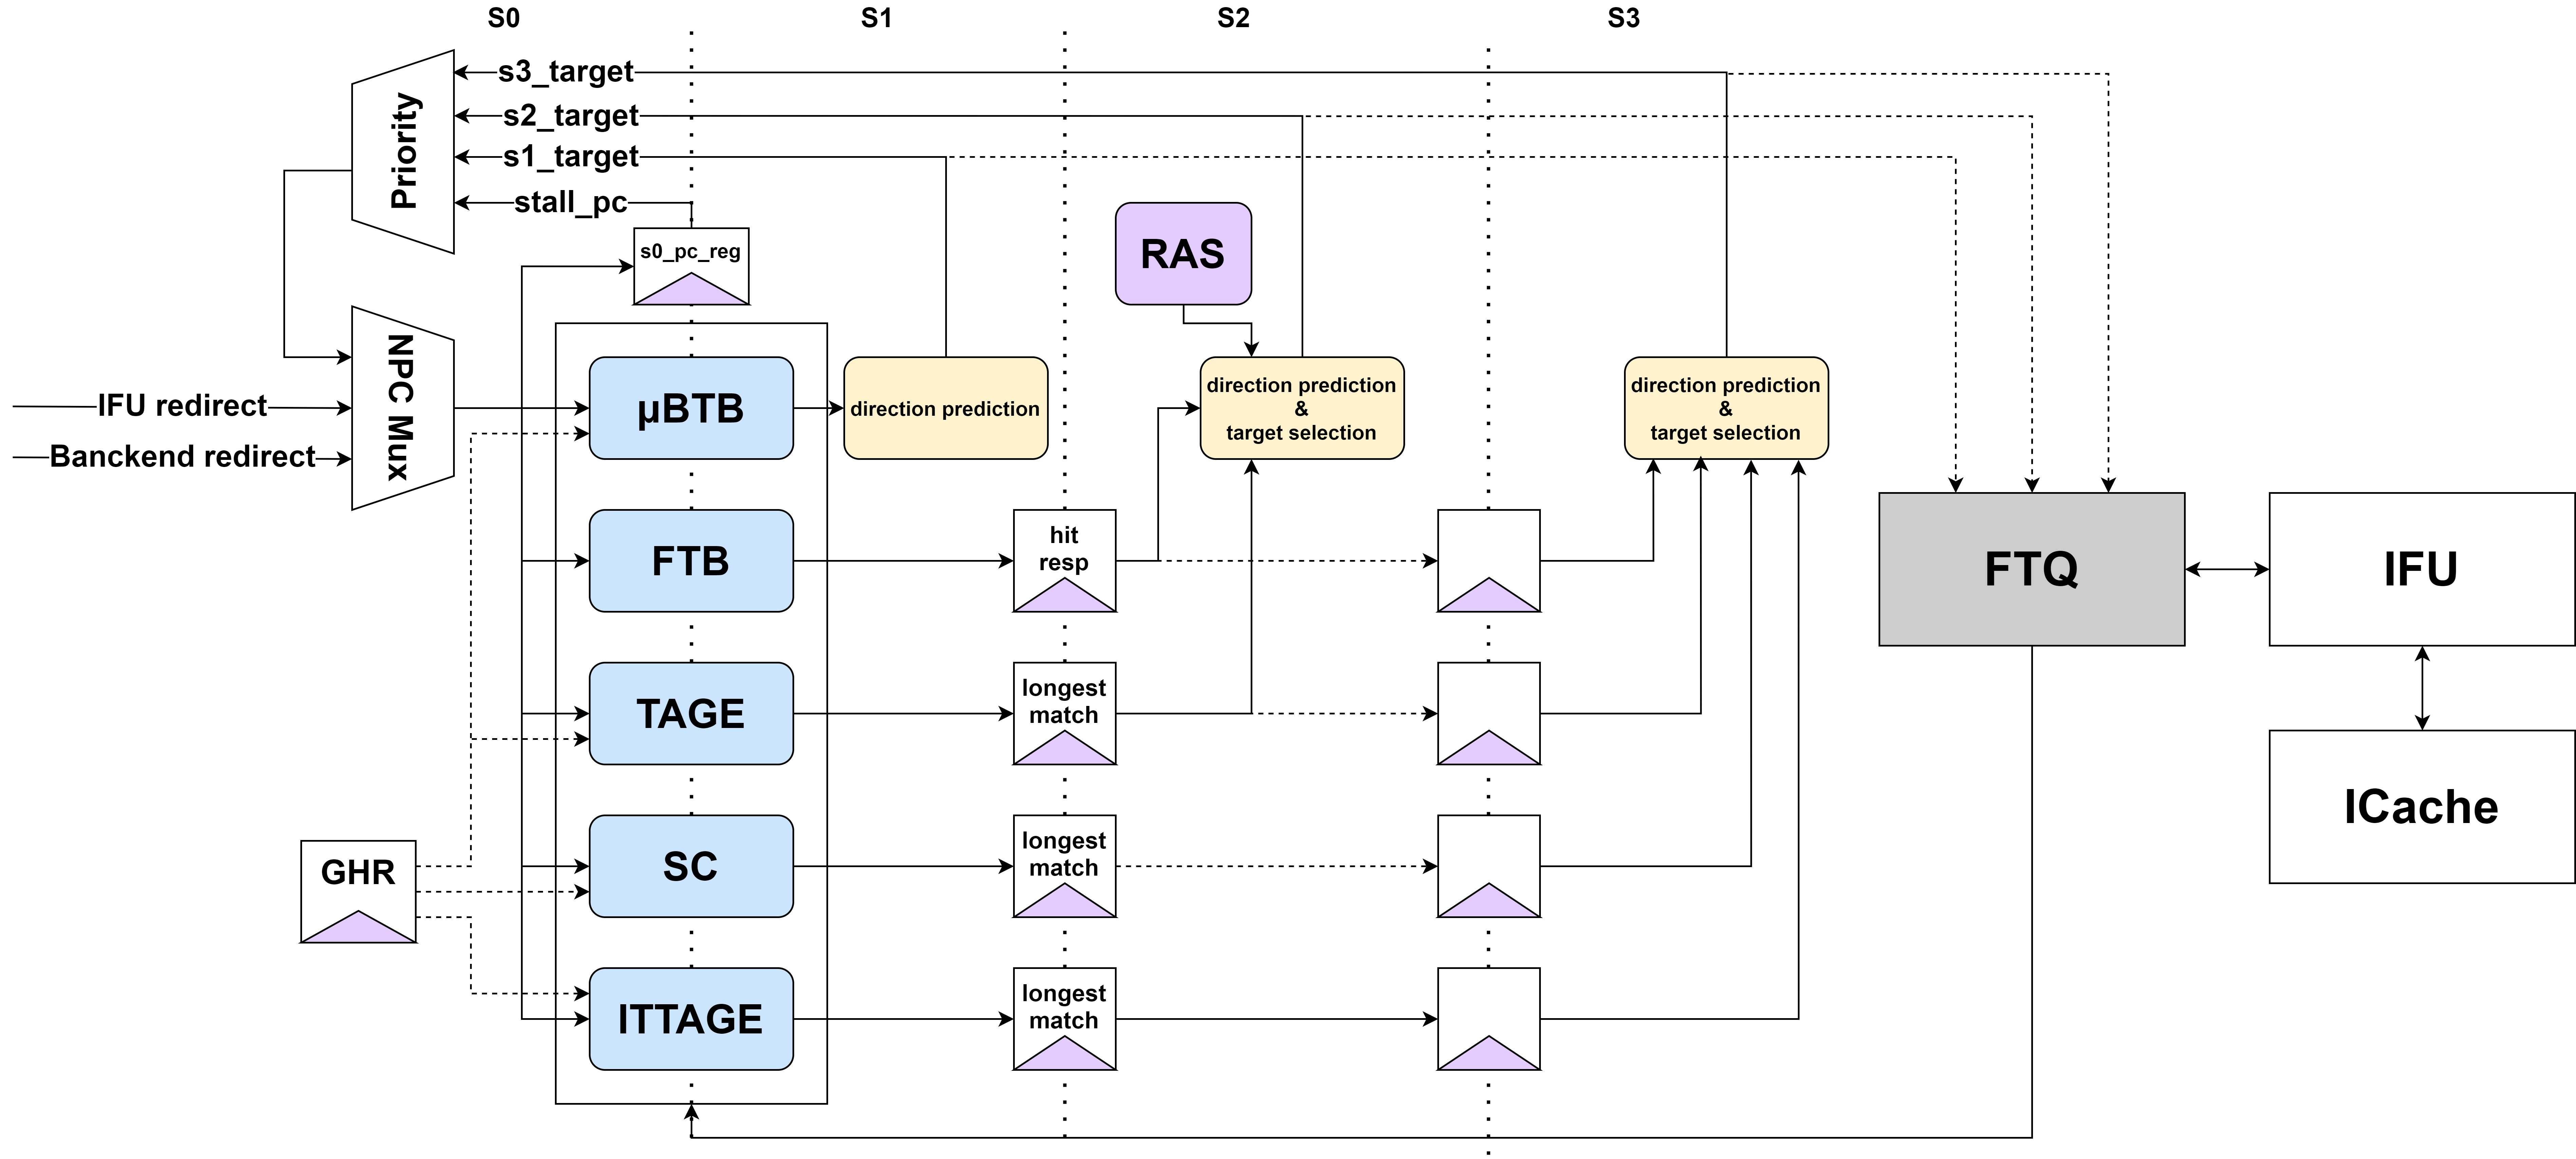
\includegraphics[width=1\textwidth]{BPU-FTQ-IFU.jpg}
	\caption{香山处理器第二版分支预测架构图}
	\label{fig:figure21}
\end{figure}

香山分支预测的主要预测器使用的是TAGE算法\cite{tage, tage-sc-l, new-case-tage},但是由于TAGE预测算法需要索引预测表,还要计算哪些表命中,最后从中选择出历史长度最长的表得出预测结果,逻辑比较复杂,需要的时间更长,超过了一个周期所需的时间。如果只使用TAGE进行预测的话,那么分支预测每2个周期才能够发出一个取指请求,显然破坏了流水线,因此为了能够让分支预测流水线无气泡的流水,需要一个逻辑比较简单,每周期都能够做出一次预测结果的预测器,也就是负责在S1做出预测的Micro BTB,它每周期都能够针对上一个周期的pc给出预测结果,及时的给出下一周期需要预测的pc,这样就能够让流水线无气泡的工作。之后S2能够得到由FTB、TAGE和RAS联合做出的预测结果,由于S2的算法更复杂,能够覆盖更多的情况,因此可以认为它的预测准确率高于S1。当出现S2的预测跳转方向和跳转目标地址和S1预测的结果不相同时,以S2的预测结果为准,这意味着之前S1预测的结果需要修正,需要清空S2之前的流水线,从S2预测的下一周期目标地址开始重新预测,这时分支预测流水线就会产生1拍的气泡。同样的,在S3会使用SC和ITTAGE再进行一次预测, 一般来说认为这次的预测是最准确的,也就是说S2的预测结果和S3预测结果不同时以S3的结果为准。当出现S2和S3预测结果不同时,也需要刷新分支预测流水线重新取指,这会带来2周期的气泡。

分支预测还需要管理分支历史,由于使用了Fetch Block作为基本分支预测单位,而Fetch Block中的特性使得在更新分支历史时有些许的不同。这部分会在第四章中详细说明。

相比于第一版的设计,第二版最重要的改动就是限制分支预测宽度和将取指功能和分支预测部分解耦,将分支预测流水线和取指流水线统一称为前端流水线,而在这之后的流水线称为后端流水线。通过重构前端,将取指单元的执行顺序移到了分支预测之后,这样做的好处在于可以减少一些前端流水线的气泡。

\section{Composer设计介绍}

参考了BOOM提出的COBRA架构,因此第二版架构中所有的预测器都继承自同一个BasePredictor基类,它们有着统一的接口,在实例化预测器时,所有的预测器都按照优先级顺序排列存储在一个components列表中。所有的预测器之间的连线和数据传输都由Composer模块负责。

除了负责连线以外,Composer模块另一个重要的作用就是为所有预测器的meta信息进行打包和解包。由于分支预测在运行时,会产生许多的预测信息,有些预测信息需要保存起来,在指令提交时取回这些信息用于恢复和训练分支预测器,这类信息统称为meta信息。而不同预测器的meta信息数量类型都不相同,为了便于存储,将每一次预测中所有预测器的meta信息都强制转换为无符号整数类型,将它们按照预测器优先级顺序拼接起来,变成一个超长的无符号整数类型,这样既方便了存储,也提高了代码的可读性。当指令提交或误预测时,再把meta信息取回,按照之前打包时的顺序,将所有的meta信息拆分开,再转为各个预测器所需要的meta信息类型,分配给各个预测器。这部分工作就是由Composer完成的。

通过使用Composer组织所有的预测器,在需要增加或减少预测器时,由于接口都是统一的,就可以免去预测器之间复杂的连线操作,极大提升了开发效率,也降低了出错的可能。虽然所有的预测器都使用统一的接口,那么对于每个预测器来说,必然有些接口是冗余无用的,但是由于Chisel的语言特性,这些没有在预测器中使用的接口,编译成Verilog代码时都会被编译程序自动优化掉,因此在生成的Verilog代码中,所有的预测器都有着自己独有的接口,不会存在冗余的情况。

\section{FTB设计介绍}

由于分支预测通常运行在取指之前,因此无法通过对指令码进行预译码来识别一条指令是否是分支指令,也无法知道一条分支指令的跳转目标地址。即使在第一版的设计中,取指和分支预测同时进行,等到将指令码从指令缓存 (Instruction Cache) 中取回时,也要等到2周期以后。由于局部性原理,执行过的分支在之后再次被执行的可能性很大,因此需要在程序执行过程中,将已经执行完毕,知道分支类型、跳转目标地址等相关信息的分支指令都保存在一个buffer中,通过它们的pc进行索引,这样下次再遇到同一条分支指令时,就可以通过查找这个buffer来获得它的相关信息,从而得知它的指令类型和跳转目标地址。这就是BTB (Branch Target Buffer) 的主要功能。它负责在预测时指出哪些指令是分支指令,以及它们对应的跳转目标地址。

在第一版设计中的BTB,以单条分支指令为基本单位,而由于前端的取指宽度是32Byte,算上4Byte长的普通指令和2Byte的压缩指令,一次取指中最多可能同时有16条分支,即16条都是压缩指令的情况,因此第一版设计中的BTB总共有16个bank,每个bank对应指令块中可能是一条分支指令的起始位置。而相对的进行分支预测时,也要同时对这16条指令进行索引和预测,再最后要从这16条预测结果中选出最终生效的一条指令,将其预测的下一周期取指pc送回S0。

在第二版的设计中,为了减少分支预测宽度,降低流水级中的逻辑门级数,采用了Glenn提出的FTB (Fetch Target Buffer) 设计\cite{scalable-frontend},相比于BTB,FTB主要的改变在于将buffer中储存的项由单条分支修改为了一个有一定约束的取指块 (Fetch Block),通过给定的约束,前端每次的取指宽度由32Byte的固定大小改为了不固定的大小,每个Fetch Block的大小由block中分支指令的分布决定,Fetch Block限制了每个block中分支指令的数量上限,在第二版设计中,限制每个block中最多只能够有2条条件跳转指令 (branch)和一条无条件跳转指令 (jump)。通过这种设计,能够将分支预测的宽度由第一版的16降低为2,从而减少最后的选择逻辑门级数,达到减少组合逻辑电路延迟的效果。在第三章中会更加详细的讨论FTB的实现。

第一版设计中,BTB总共有2K项,16个bank,2路组相联。第二版中FTB虽然也有2K个项,4路组相联,但是由于一个FTB表项所占的空间几乎等于原来BTB一个表项的2倍,因此实际上第二版实现FTB所使用的SRAM大小应该是翻倍了的,这会带来一定的性能提升,同时会增大分支预测部分的面积。

\section{Micro BTB设计介绍}

Micro BTB作为一个小型的预测器,需要在每周期内都得出一个初步的预测结果,来保证分支预测流水线的连续。因此首先具有一个小型FTB的功能,它也能够保存分支指令的信息,但是由于它需要在很快的时间内做出一个初步的预测,因此它的逻辑必须简单,使用的硬件资源必须足够小,因为过于复杂的逻辑和过多的面积都会导致它无法按时给出预测结果。

在第一版的设计中,Micro BTB就是一个小型的BTB,并且自带了一组两位饱和计数器,有16个bank,每个bank中可以存储16条分支指令的信息,按照全相联存储。在预测时通过索引分支指令信息,并且以两位饱和计数器的值来给出预测结果。由于存储的信息很少加上预测算法简单,因此Micro BTB的预测速度非常快,当拍就可以给出预测的结果。

在第二版的设计中,由于需要满足更高的频率要求,Micro 由原来的全相联修改为了256项直接映射,使用SRAM实现。直接映射在索引和判断命中时能够有更短的电路延迟,且使用单口的SRAM在面积上也不会比第一版的寄存器堆大太多。另外去除了原来的两位饱和计数器组,修改了Micro BTB的预测算法,首先使用要预测的pc和全局历史哈希做索引,当Micro BTB命中,即发现当前pc对应的取指块已经被保存时,它会依据上一次索引到该项的分支的跳转方向,以此作为这次的预测结果。这种逻辑会比更新和计算饱和计数器更加简单,同时不会有太大的性能损失。

\section{RAS设计介绍}

RAS (Return Address Stack) 是一个专门针对call和return指令优化的预测器。知道在程序中往往存在着大量的函数,它们会不断地调用和返回,指令执行过程如图\ref{fig:figure22}所示,通常程序执行某个函数时,首先会使用一条call指令跳转到函数的起始地址,然后从起始地址顺序往下执行,当函数执行完后,最后会有一条return指令,再将程序跳转回call指令之后的下一条指令继续执行。当然在执行函数的过程中也有可能继续调用一个新的函数。由于函数调用是递归的,因此可以使用一个栈结构来保存所有函数调用的返回地址。当检测到一条call指令时,将这条call指令之后的下一条指令存入RAS,然后当检测到一条return指令时,就将RAS栈顶保存的地址出栈,作为这条return指令的跳转目标地址。

\begin{figure}[htb]
	\centering
	\setlength\tabcolsep{3pt}  % 同一行中的图片间隔
	\vspace{5pt} % 图片上部的空白,如果太小的话,图片顶部会与正文内容十分接近
	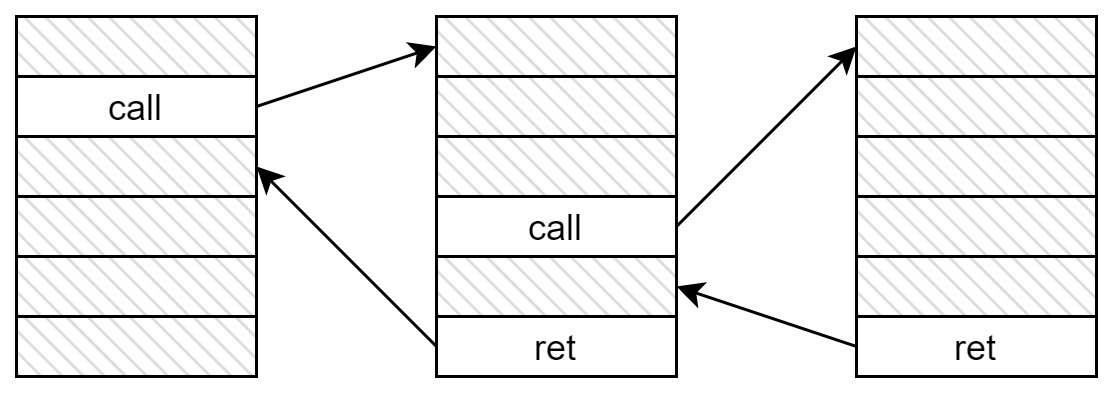
\includegraphics[width=0.8\textwidth]{function-call-ret.jpg}
	\caption{在程序中函数的调用和返回}
	\label{fig:figure22}
\end{figure}

由于程序中有大量的类似于递归调用的行为,即有的函数在满足条件时,会不断地自己调用自己,在这种情况下,每次要保存的返回地址起始都是相同的。因此每个RAS项都带有一个计数器,当这一次调用的返回地址与栈顶元素的返回地址相同时,就不会将这次调用入栈,而是给栈顶元素的计数器加1。同样的在return指令时,首先会检测栈顶元素的计数器,如果计数器大于1,则不弹出栈顶元素,只是将栈顶元素的计数器减1,直到计数器为1时才出栈。

这样修改能够减少RAS在遇到某些特别深的递归时,不至于一直入栈相同的返回地址,导致栈溢出,能够提高RAS的预测准确率。

而为了减少预测时读取RAS的延迟,另外使用了一个专门的寄存器用来存储当前栈顶的地址副本,在每次RAS入栈出栈时也会同时维护这个副本。当检测到一条return指令时,就可以直接使用这个单独的寄存器,而不用从整个RAS栈中读取栈顶元素,能够节省从RAS栈中索引出栈顶元素所需要的时间。

RAS在分支指令出现误预测时需要恢复,不然可能会出现地址错乱的情况,RAS在误预测时修复的方法有很多种\cite{ras-recovey, ras-revisited},而第二版实现时使用了一种较为简单的恢复方法,即在分支预测时将当前的栈顶指针和栈顶元素保存起来,在恢复时只恢复栈顶元素和指针,这样一来既能够简化恢复逻辑,也不会带来过多的误预测。

\section{TAGE设计介绍}

TAGE (TAgged GEometric history length branhc predictor) 是由André提出的一种预测器\cite{tage},曾经多次夺得过分支预测大赛 (CBP, Championship Branch Prediction) 的冠军,之后由许多研究者对其不断地优化和改进,是目前公开的分支预测性能最好的预测器之一。TAGE是一个使用全局历史索引的方向预测器,也就是说它只会用来预测分支是否跳转,而跳转目标地址需要由FTB、RAS或ITTAGE来提供。


\begin{figure}[htb]
	\centering
	\setlength\tabcolsep{3pt}  % 同一行中的图片间隔
	\vspace{5pt} % 图片上部的空白,如果太小的话,图片顶部会与正文内容十分接近
	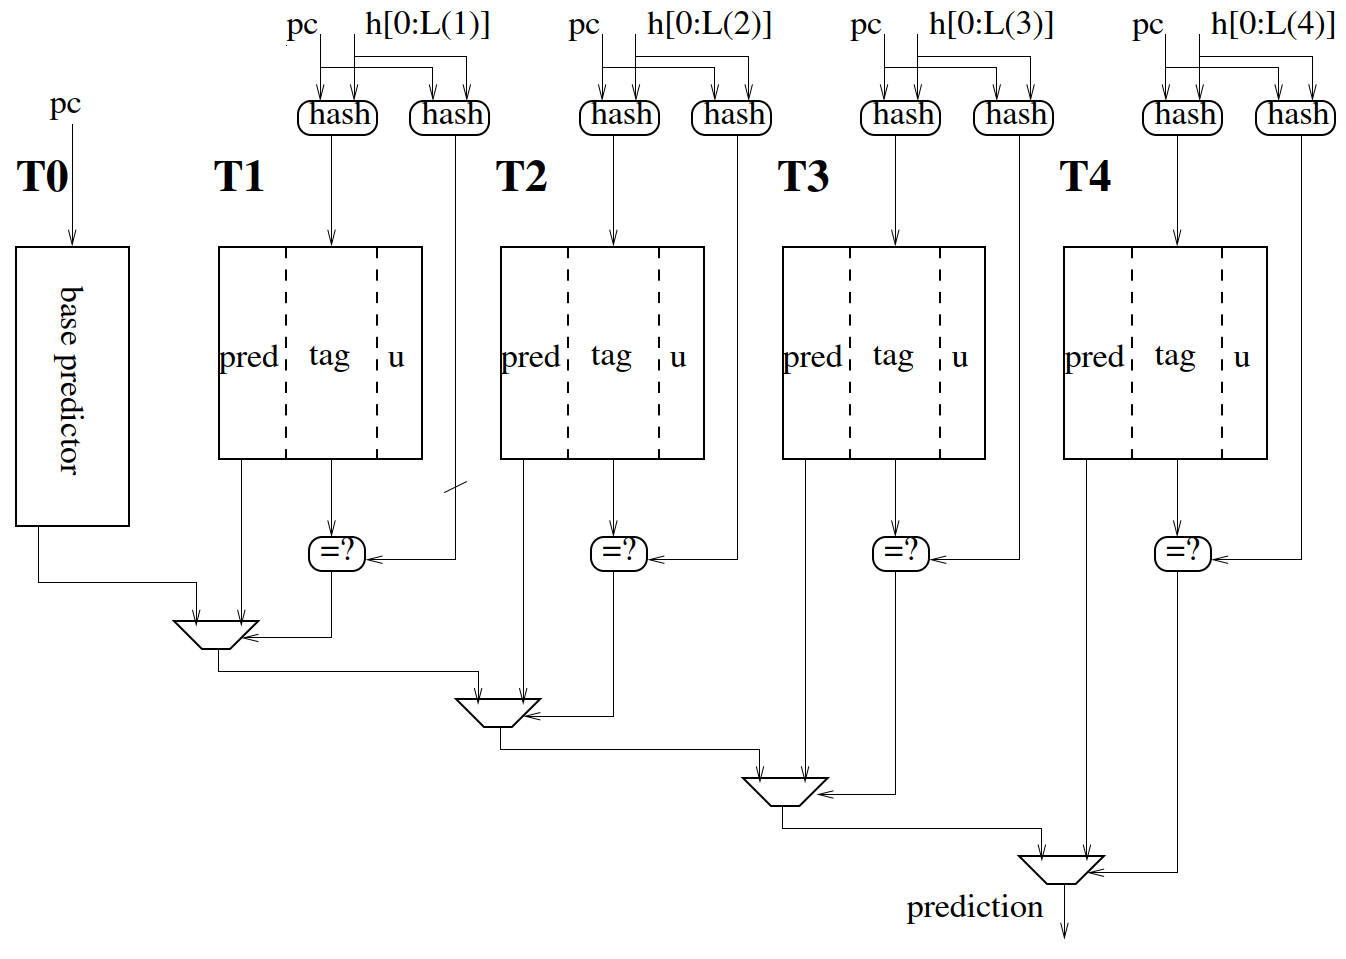
\includegraphics[width=1\textwidth]{tage.jpg}
	\caption{TAGE预测器结构图\cite{tage}}
	\label{fig:figure23}
\end{figure}

TAGE预测器由一个基本表T0,和n张预测表Ti (i=1,2,3,...,n) 组成,其中基本表是一组使用SRAM存储的2位饱和计数器。而每张预测表的单个表项中都有一个valid位,一个tag,以及一个3位饱和计数器。每张表的大小,用于索引的折叠历史长度,以及tag长度都是可配的,通常来说从T1到Tn,用于索引的折叠历史长度程几何递增关系。第二版的TAGE表配置如表\ref{tb:table21}所示。

\begin{table}[]
	\caption{香山第二版分支预测架构TAGE预测表配置}
	\label{tb:table21}
	\centering
	\begin{tabular}{|c|c|c|}
		\hline
		项数   & 历史长度   & tag长度   \\ \hline
		4096 & 8 & 8 \\ \hline
		4096 & 13 & 8 \\ \hline
		4096 & 32 & 8 \\ \hline
		4096 & 119 & 8 \\ \hline
	\end{tabular}
\end{table}

在使用TAGE做预测时,需要知道待预测指令的pc,以及当前的分支全局历史,由于全局分支历史是一个较长的bit串,所以先使用简单的哈希算法将其折叠,然后再与pc一起计算出一个值,使用这个值去索引预测表,由于不同的预测表使用的折叠历史长度不同,因此相同的pc和全局历史在不同的预测表中也会映射到不同的表项中。

在索引到每张预测表中的表项后,首先会检查这个表项是否valid,如果是valid,那么继续比对其中存储的tag与pc是否匹配,如果匹配了则代表这张表命中了,选择该表项的饱和计数器作为这张预测表的预测结果。在多张预测表命中时,TAGE会选取折叠历史长度最长的那张表的预测结果,作为整个预测器的预测结果,这个表成为provider。而如果T1到Tn都没有命中,则会使用T0基本表中的饱和计数器作为预测结果。

而如果发现provider中的表项是新写入的,其中的值还是写入时的初始值,可以认为这个表项是还没有训练完成的,因此TAGE在查找所有命中的表中最长历史的表时,也会同时查找第二长历史的表,称为alrProvider如果发现匹配的最长历史表中的计数器是初始值的话,就会使用匹配的第二长历史表的预测结果。

但是为了优化时序,减少路径延迟,在第二版的设计中一律将altProvider设为T0的预测结果。

% 更新逻辑

在有分支指令从后端发来更新时,首先需要检查之前这条分支预测时是否有预测表命中,如果有命中的表,就会更新对应的表中的表项里的饱和计数器,如果分支跳转则饱和计数器加1,不跳转则饱和计数器减1。

% 分配新项
当一条分支发来更新时,如果它命中的表Ti不是Tn,则会去选择一张表Tj (i<j<=n),且u标志位为false的项分配,从Ti+1到Tn查找,选择第一张符合要求的表进行分配,新分配的表项的饱和计数器根据这条分支的跳转方向来决定,如果跳转则置为weak taken,否则置为weak untaken。

u标志位用于在分配新的表项时来决定分配给哪一张表,u位在一条分支指令最终预测正确,但是它的altProvider预测结果是错误时增加,当所有的u都为true时,还有新的项要写入,则复位计数器tick递增,否则递减,当到达一定的值时,就会把所有的u都复位。

由于在一条分支指令从预测到更新之间有一定的延迟,而这段时间内这条分支对应的表项有可能会有其他的写入,因此在实现时借鉴了BOOM中的wrbypass技术,通过一个简单的buffer,记录最近的TAGE写入,这样在更新饱和计数器时,首先去查找wrbypass中有没有对应的表项,如果有,就以wrbypass中存储的饱和计数器为基础去更新,如果没有就使用从后端传回来的meta信息中的饱和计数器去更新。

在第一版的设计中TAGE的基本表直接复用了BIM (Bi-Model Predictor),而在第二版中为TAGE添加了单独的基本表,主要原因是在第二版的设计中S2就能够得到TAGE的预测结果,因此,不需要BIM。其次就是TAGE的基本表的更新策略和BIM有些许的不同。

% TAGE由多张预测表组成,每张表通过不同长度的分支历史来索引,表中的每一项都是一个饱和计数器。每次预测时会同时查找所有的表,然后从中选择出历史长度最长且tag匹配的表,以它的饱和计数器值作为分支预测的结果。

\section{SC设计介绍}

SC (statistical corrector) 是TAGE预测器的一个组件,如图\ref{fig:figure24}所示。主要针对的是对某个方向只有很小的偏差,但是与历史路径相关性不强的分支\cite{tage-sc-l, isl-tage}。这种类型的分支有时TAGE无法准确预测。

SC也是由几张表组成的,每张表中的表项有2个6位的计数器,一个用于在TAGE预测跳转时使用,一个用于TAGE预测不跳转时使用。在预测时会根据带预测指令的pc和折叠历史进行哈希索引。将每张表索引出来的计数器的值相加,再加上TAGE预测的结果。然后使用最终的和与某个动态变动的阈值进行比较,再通过TAGE的预测结果进行一个二选一,得出最后的预测结果。

在预测时SC会有一个动态的阈值,这个阈值会动态的改变,每次会根据待预测指令的pc和历史索引每个表,将得到的结果相加,当相加的结果大于阈值时就翻转TAGE的预测结果。

Threshold自身有一个5位的计数器,每次有指令更新时,如果SC曾经做出过预测,且满足一定条件时进行更新。而阈值也会根据新更新的计数器计算,如果饱和计数器达到最大值,且当前的threshold小于最大值,则增加;当饱和计数器达到最小值,且当前的threshold大于最小值,则减少。

% 每次预测时SC会收到待预测指令的pc,分支历史,以及TAGE做出的预测结果。SC会索引每一张表,并取出每张表对应的两个饱和计数器,最后将它们相加,再加上TAGE的饱和计数器,得到一个totalSum。当TAGE命中且,totalSum相加大于0,且大于当前的threshold,或相加小于0,且相加小于负的threshold时,SC会做出预测,预测方向为所有SC表取出饱和计数器之和是否大于0.通过TAGE预测是否跳转来选择用0还是1。

与TAGE类似,SC也有wrbypass的结构,用来保证在指令从预测到更新期间有其他的指令更新了相同的表项,保证了用于更新的计数器是最新的值。

\begin{figure}[htb]
	\centering
	\setlength\tabcolsep{3pt}  % 同一行中的图片间隔
	\vspace{5pt} % 图片上部的空白,如果太小的话,图片顶部会与正文内容十分接近
	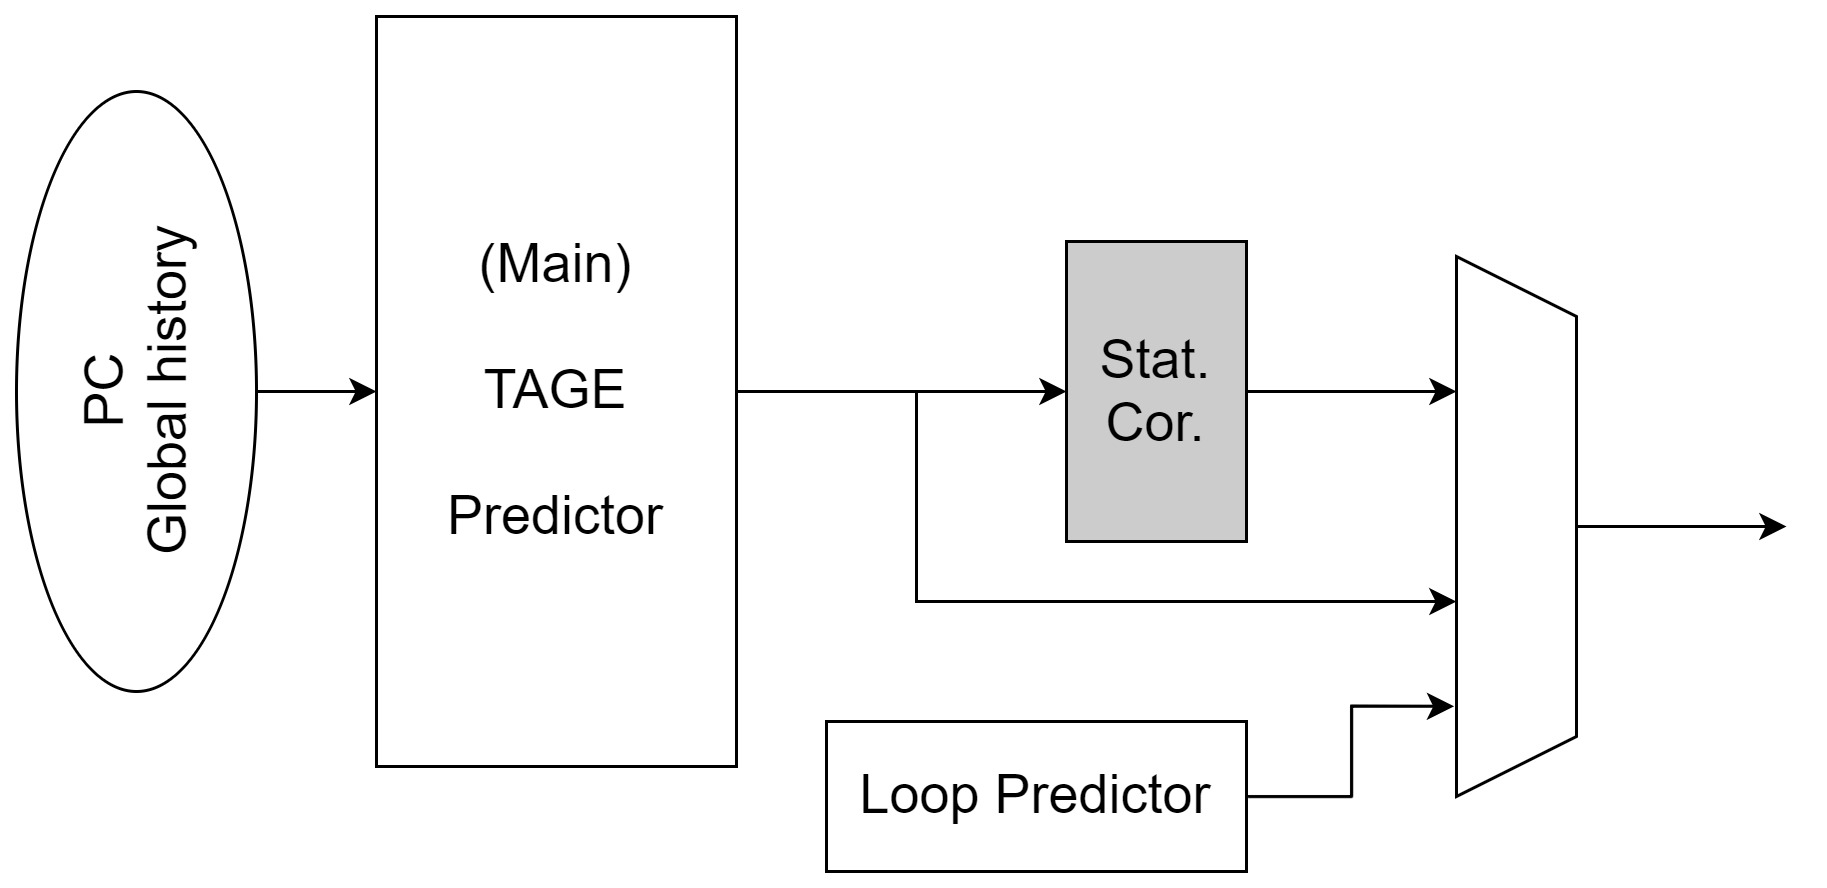
\includegraphics[width=1\textwidth]{sc.jpg}
	\caption{TAGE-SC-L架构图\cite{tage-sc-l}}
	\label{fig:figure24}
\end{figure}

% 还有那个算threshold的算法

\section{ITTAGE设计介绍}

ITTAGE (Indirect Target TAgged GEometric history length branhc predictor)\cite{tage, ittage} 是一个专门针对间接跳转分支的预测器,也是由André提出的,其算法大部分与TAGE相同。不同之处在于TAGE中用于判断跳转方向的饱和计数器被替换成了一个跳转目标地址和一个置信度计数器,在预测时通过pc和分支历史索引到的表项返回,如果这条分支被预测跳转,则作为这条分支的跳转目标地址。

\section{分支历史管理策略}

在分支预测中分支历史管理也是一个重要的功能。在第一版的设计中,参考了BOOM,将每个32Byte的取指block视为整体,每个block在全局分支历史中占用1bit,无论其中有多少条指令。在更新分支历史时通过寄存器移位来更新分支历史,误预测恢复时也是直接将之前保存的完整分支历史覆盖回全局历史寄存器中。

而在第二版架构中,为了令全局分支历史更加准确,改为了每一条分支指令在全局历史中占用1bit,这样的话全局分支历史的管理策略就需要做相应的改动,为此设计了新的分支历史更新逻辑,在需要更新分支历史时,需要判断当前Fetch Block中有多少条需要加入到分支历史中的分支指令。此外第二版中还将原来的寄存器移位更新改为了使用分支历史指针来管理更新,在误预测恢复时也是直接传回误预测指令所对应的分支历史指针做恢复逻辑。

在第二版的架构中除了保存完整的分支历史以外,还保存了用于索引TAGE、ITTAGE等预测器所需要的折叠分支历史,不同于第一版,每次需要使用折叠历史时都是用完整的分支历史计算,这次的这叠分支历史是直接按照折叠的状态来维护的,这样能够得到更好的时序结果。

在分支预测时,S0的分支历史会顺着流水级一级级往下传,确保每个流水级预测时使用的都是相同的分支历史,同时每个流水级也会生成根据自己本身预测结果更新过的分支历史,S0分支历史寄存器的历史会通过一个优先选择器,选择合适的新分支历史来源进行更新。

\section{本章小结}

本章首先详细介绍了本文提出的分支预测架构的流水线设计和工作流程,给出了架构图,展示了每个预测器在流水线中的不同位置。之后单独列出了Composer模块,以及FTB,Micro BTB,RAS,TAGE等预测器的功能和算法。其中主要介绍了TAGE预测器的功能逻辑,以及相对于第一版架构做出的改进。为之后两章的内容做了铺垫。
% !Mode:: "TeX:UTF-8"
\chapter{限制分支预测宽度的改进策略}

本章首先介绍香山雁栖湖架构的取指策略,接下来介绍在高性能处理器中,按照指令地址对齐的取指策略,和不对齐的取值策略的优缺点.并指出为什么需要限制分支预测的宽度,过宽的分支预测宽度会对处理器整体设计带来怎样的影响。最后介绍在南湖架构中,修改取指策略,限制分支预测宽度相关技术的实现。具体有FTB表项的数据结构设计,以及FTB更新和管理策略,并解释了为什么要这样设计。通过修改每拍取指的基本单位,实现了限制前端在一次取指内容中分支指令的上限。

\section{香山雁栖湖架构取指策略}

在不同的处理器中,有许多种取指策略。例如在香山雁栖湖架构的设计中,取指pc是按照32Bytes对齐的,也就是低5位都为0,每次取指固定取32Bytes的指令数据。这种对齐取指设计好处在于可以有效避免在一次取指中指令跨Cache行的情况,取指单元每次取指只需访问一个Cache行。而这一点在南湖架构的设计中已被修改,南湖架构的取指单元在每次取指时最多可以同时取出2个Cache行的数据。其次就是由于指令都是对齐的,因此一条指令在整个取指的block中的位置是固定的,由低5位决定。这样可以保证在进行分支预测时,每条分支指令都只会被预测器的同一个bank预测、记录和更新,不会出现同一条指令在不同bank的情况。而南湖架构的设计中的取指不再对齐,也因此有可能出现同一条分支指令保存在不同的表项中的情况,这在某种程度上会降低预测器存储空间的使用效率。

但是按照指令地址对齐取指也有一些弊端,首先如果某次取指的起始pc非常靠近其所在的Cache行的末尾,由于取指单元不能够跨Cache行取指,则这次取回的有效指令数量就不满32Bytes,一定程度上会降低取指的带宽。其次也是决定在南湖架构中修改这个机制的最主要的原因,由于香山实现了RISC-V的C扩展,即压缩指令集,RISC-V正常的一条指令 (RVI) 占4个Bytes,而C扩展中规定了许多压缩指令 (RVC),这些压缩指令只有2个Bytes长。增加了压缩指令之后,会带来一些问题,首先即使取指是按照32Bytes对齐,仍然会出现需要跨行取指的情况,如图\ref{fig:figure31}所示,为便于表示,以一个cache行 8Bytes为例,实际设计中一个cache行会大得多。图\ref{fig:figure31}(a)是不带压缩指令的情况,所有指令都是对齐的,不会出现一条指令在两个cache行中各存一半的现象,但是加入了压缩指令之后就会出现图\ref{fig:figure31}(b)的这种情况,即由于加入了压缩指令,非压缩的指令无法对齐,就会出现一条非压缩指令被2个相邻的cache行截断的情况。这种情况不光适用于RISC-V架构的处理器,所有使用有压缩指令定义的指令集架构的处理器都会有类似的问题。

当出现这种情况时,就会导致最后这条分支指令无法在一个周期内被完整取出,如果这条被截断的指令正好是条分支,便只能等到下一周期取到后半条指令码后再进行预译码操作。

\begin{figure}[htb]
    \centering
    \setlength\tabcolsep{3pt}  % 同一行中的图片间隔
    \vspace{5pt} % 图片上部的空白,如果太小的话,图片顶部会与正文内容十分接近
    \begin{tabular}{ccc}
        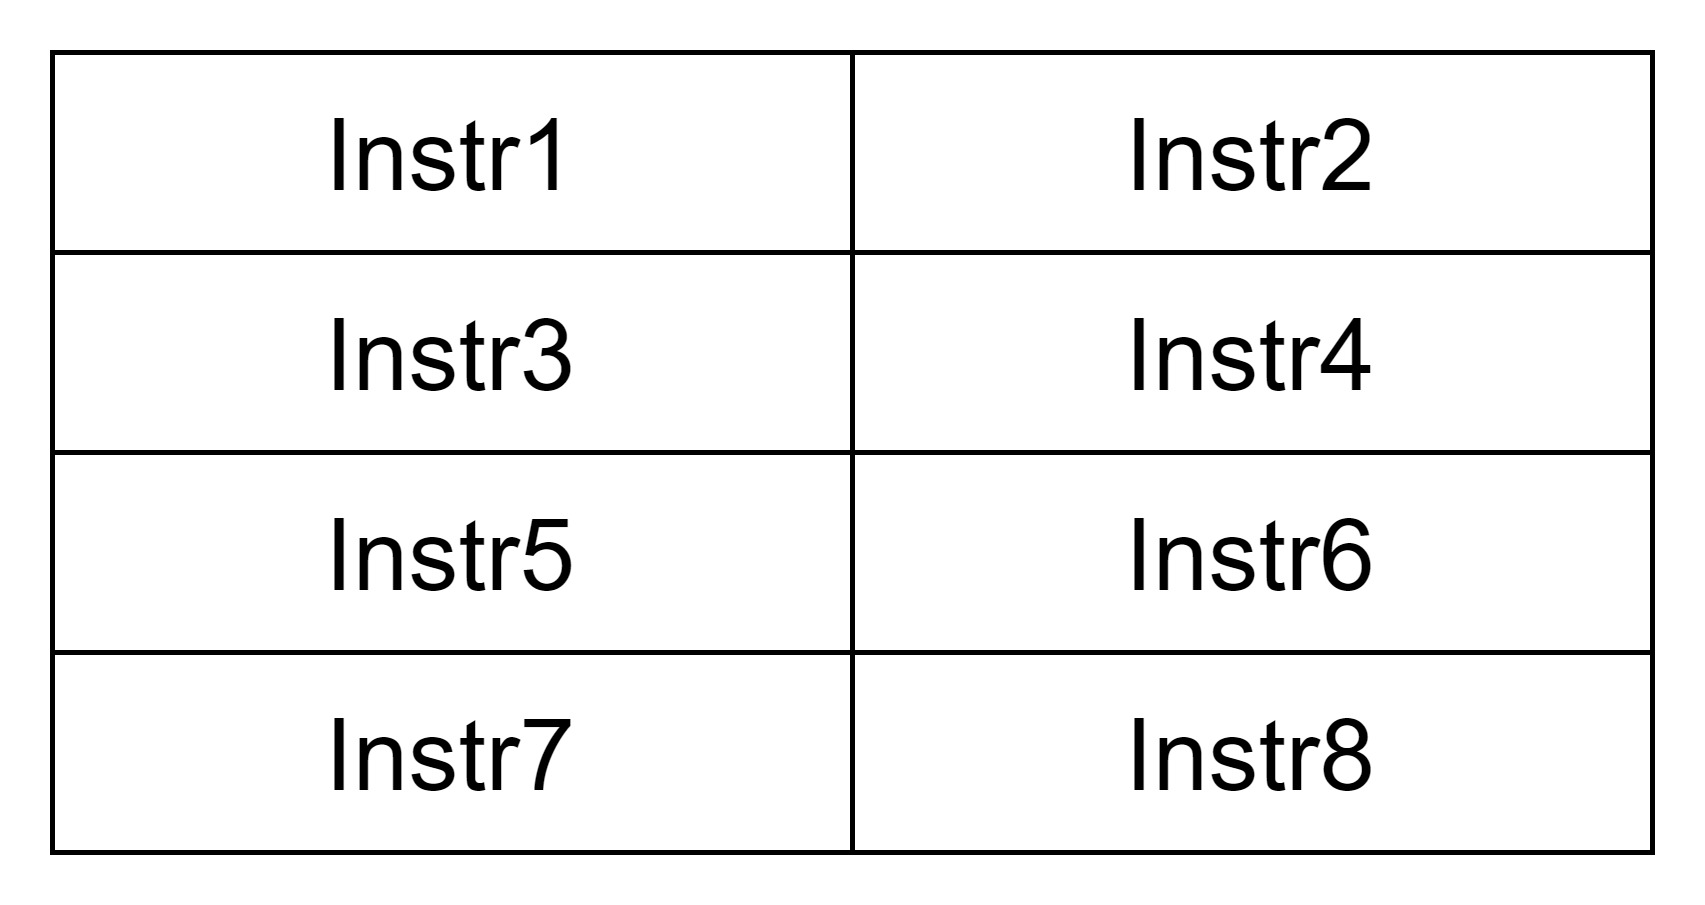
\includegraphics[width=0.30\textwidth]{RVI-only.jpg} &
        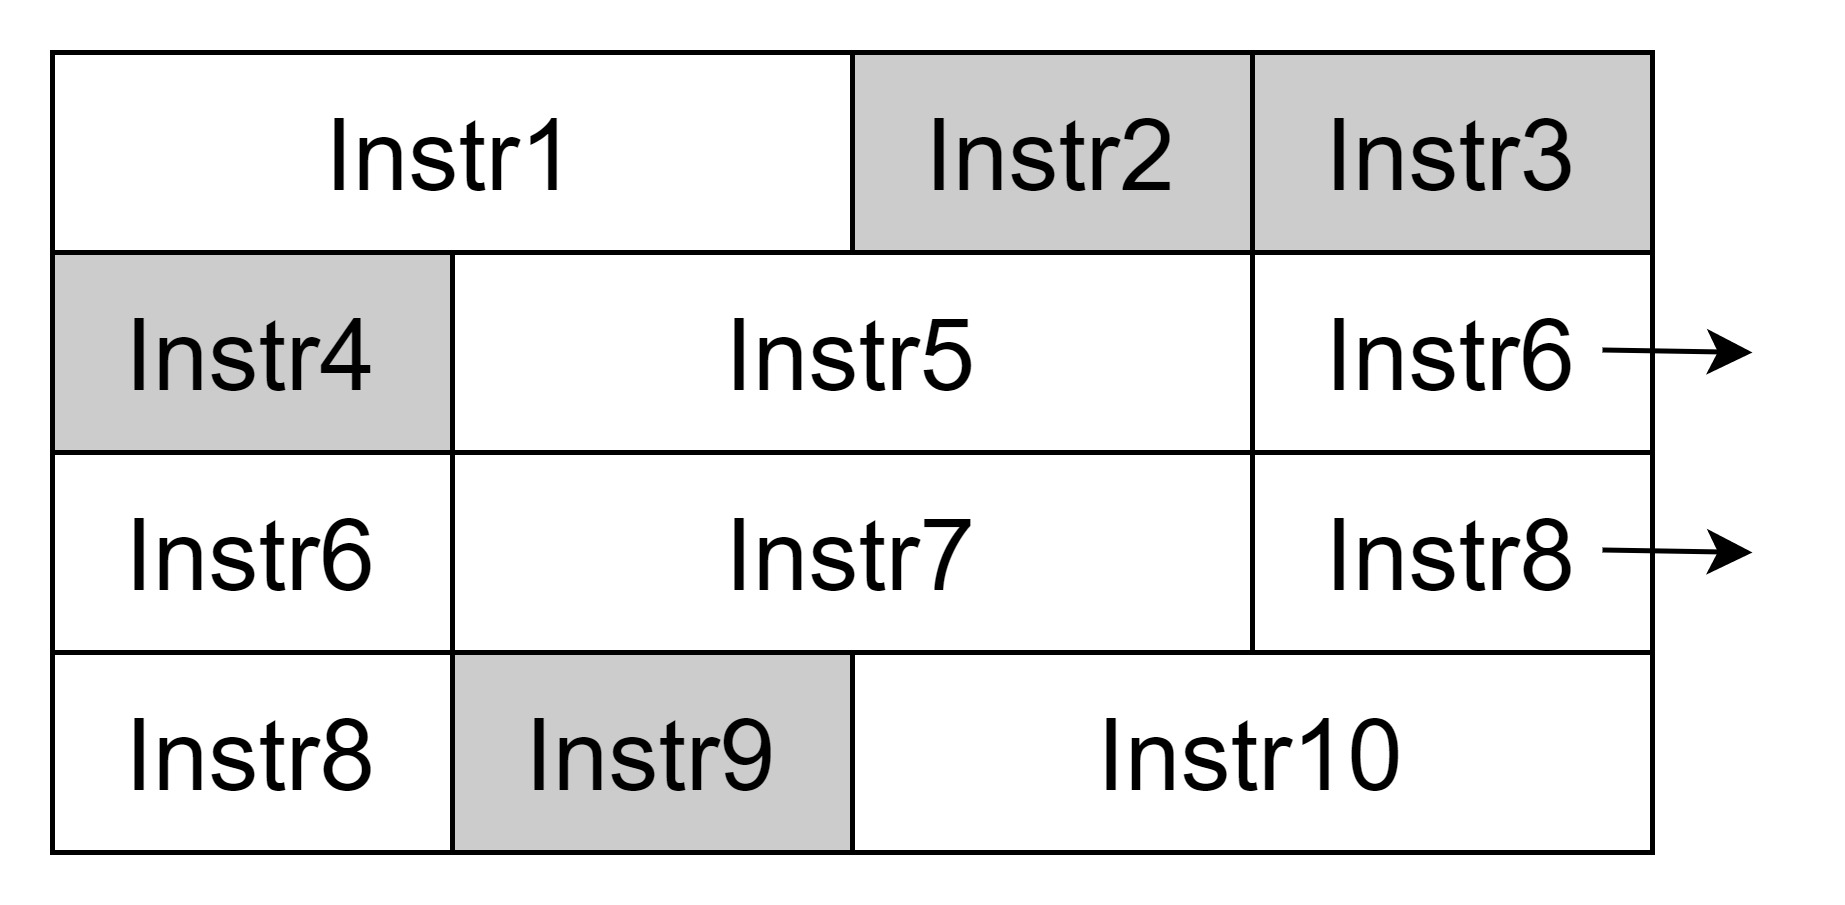
\includegraphics[width=0.325\textwidth]{RVIC.jpg} &
        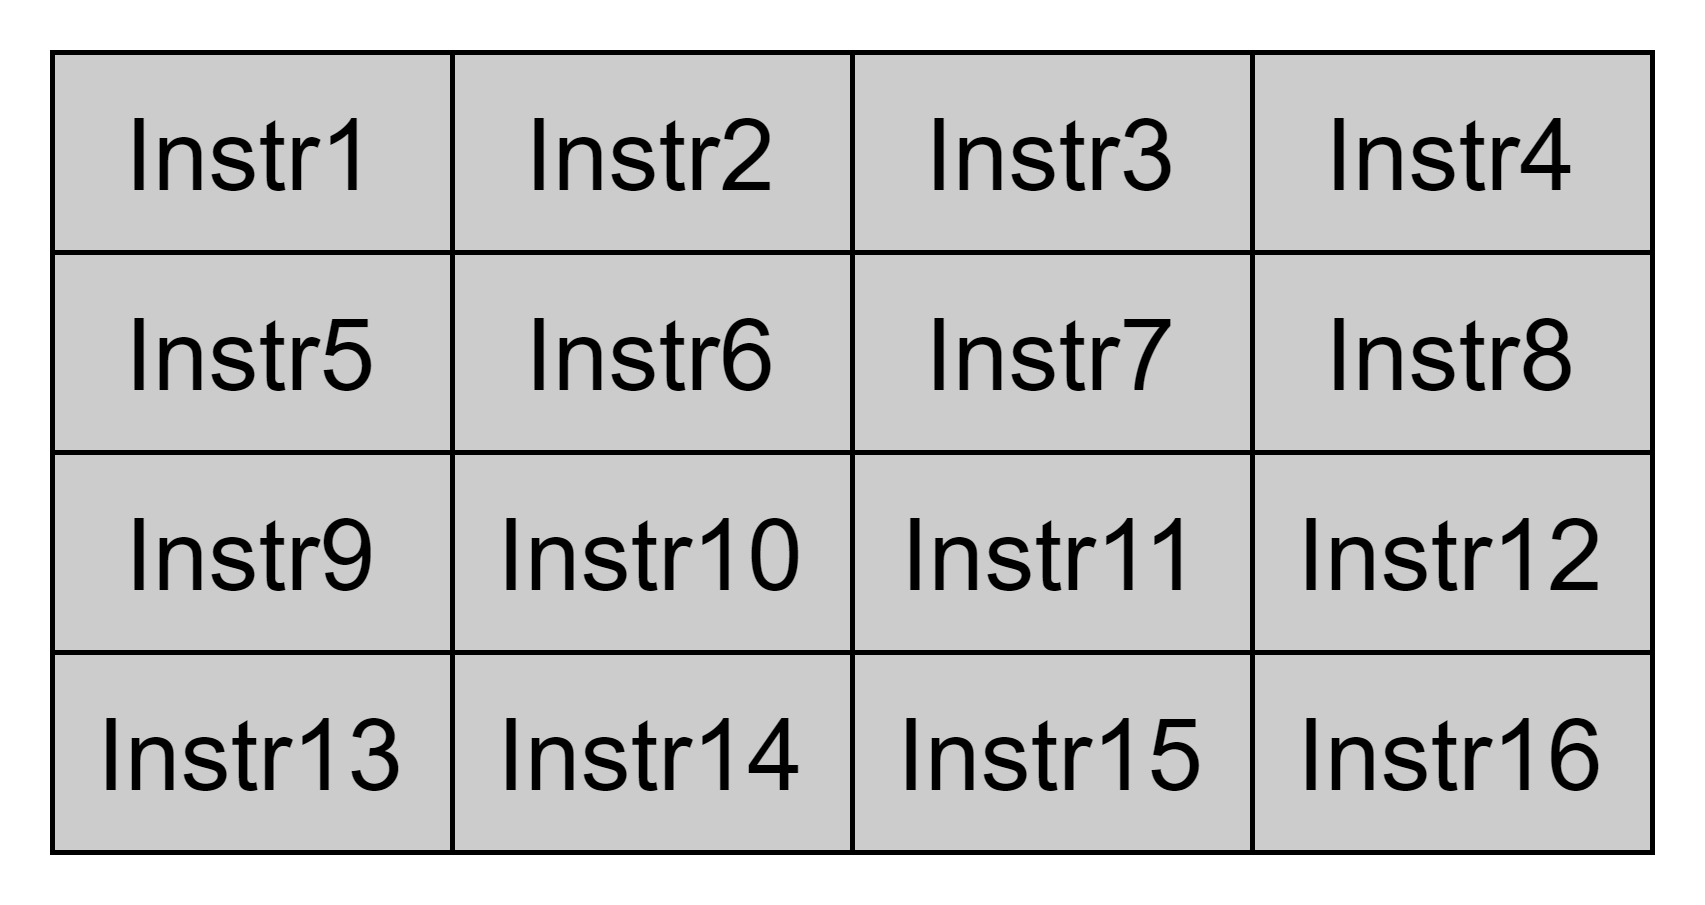
\includegraphics[width=0.30\textwidth]{RVC-only.jpg} \\
        (a) 只有RVI指令 & (b) RVI,RVC指令混合 & (c) 只有RVC指令 \\[1ex]
    \end{tabular}
    \caption{在cache行中以不同形式储存的指令码,其中白色的代表非压缩指令RVI,灰色的代表压缩指令RVC,图(b)中第6和第8条指令出现跨cache行情况}
    \label{fig:figure31}
\end{figure}

加入了压缩指令之后,如果以32Bytes为单位取指,每次取出来的数据中会有8到16条指令不等,最多的情况如图\ref{fig:figure31}(c)所示,即16条都是压缩指令的情况。因此为了能够覆盖到所有情况,香山雁栖湖架构的分支预测设计中,所有的预测器,包括雁栖湖架构中FTB的原型BTB (Branch Target Buffer) 都是以16为宽度来设计的,也就是说每个预测器都有16个bank,每个bank对应32Bytes中所有有可能是一条分支的位置。

但实际上真正在程序运行中,一次取出的指令中有这么多条分支指令的情况非常少见,这种设计在一定程度上是冗余的,意味着所有的分支预测逻辑的连线和复杂度都会大大增加,尤其是在分支预测决定最终的预测结果,给出下一周期需要预测的pc的时候,需要从预测器16个bank的预测结果中选出一条最终预测跳转的分支,从16个备选的跳转目标地址中选出一个最终的地址,这是一个4级的多选操作,而这个逻辑处于整个分支预测的关键路径上,许多的组合逻辑电路都要经过这段逻辑,因此降低分支预测宽度,能够减少分支预测的组合逻辑复杂度,减少选择最终预测结果的逻辑门数,如图\ref{fig:figure33}所示,最终达到优化时序,提高频率的效果。除了香山处理器外,在IBM zEC12\cite{ibm-zec12},龙芯\cite{loongson}等公司的商业处理器的相关论文和文档中都提到了有限制分支指令最大数量的相关技术,是目前高性能处理器领域的一个主流趋势。

\begin{figure}[htb]
	\centering
	\setlength\tabcolsep{3pt}  % 同一行中的图片间隔
	\vspace{5pt} % 图片上部的空白,如果太小的话,图片顶部会与正文内容十分接近
	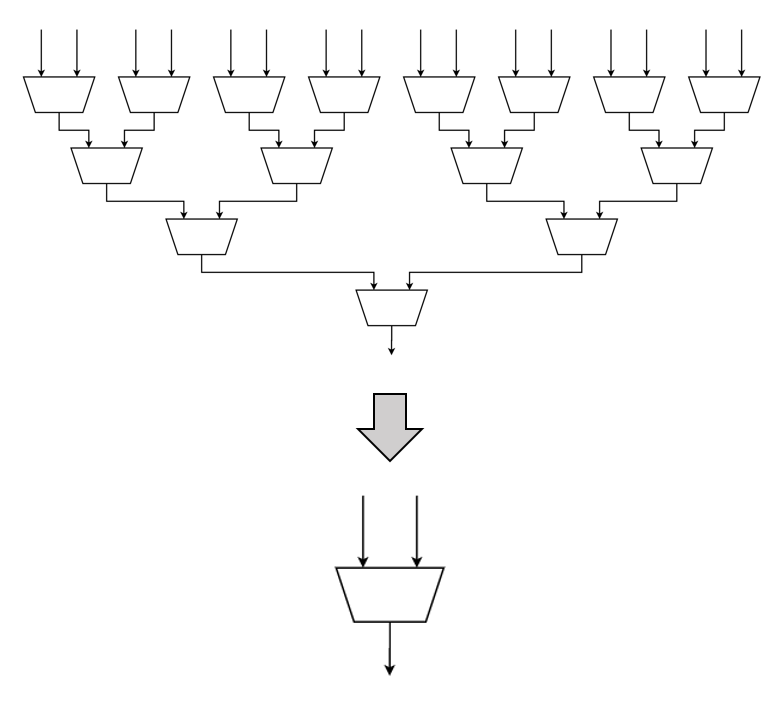
\includegraphics[width=0.7\textwidth]{mux.png}
	\caption{降低分支预测宽度后,选择最终生效分支指令的选择逻辑门层数变少}
	\label{fig:figure33}
\end{figure}

\section{Fetch Block的定义}

为降低分支预测宽度,一个思路是限制每次取指所能包含的分支指令的最大数量,因为分支预测最终的宽度是以可能的最大分支数量为准,例如上文提到的如果一次最多会有16条分支,那么分支预测宽度也必须为16,即使大部分时候并没有这么多分支。
假设将分支预测的宽度限制为2,之前的取指是以32Bytes定长为单位取指的,而在一些分支指令密集的程序片段中,32Bytes大小的指令块中大概率会出现超过2条分支,因此不能够继续以固定的大小作为取指的基本单位,需要定义一个新的基本单位,为这个单位添加一些约束条件,以此来限制每次取指的分支指令数量。

在南湖架构的分支预测架构中,定义了Fetch Block,这个概念是Glenn\cite{scalable-frontend}提出的,Fetch Block的定义如下,每个block都必须满足这三个约束条件:

\begin{enumerate}
    \item 每个block的最大大小为32Bytes,即当一段指令中没有分支指令时,仍然需要限制block的最大大小,因此规定block的最大大小和雁栖湖架构相同,都是32Bytes。
    \item 当遇到第n+1条条件跳转指令 (branch) 时,无论block大小有没有32Bytes,这个block在第n+1条branch指令之前截止。为什么不是在第n条指令后就立即截止,是因为这样就可以保证,在block中最多只有n条分支的前提下,每个block中的指令数量尽可能多。
    \item 当遇到无条件跳转指令 (jump) 时,无论block大小有没有32Bytes或有没有达到n条branch指令的上限,这个block都在这条jump指令后截止。这是因为jump指令必然是跳转的,因此在这条指令之后下一周期需要预测的pc应该由预测器给出,无论下一周期从哪里开始预测,都将会是另一个block。因此如果block中含有jump指令,必定是block中最后一条指令。
\end{enumerate}

通过以上的3条约束,就能够保证单个的Fetch Block中,branch指令不超过n条,且最多只有一条jump指令。而在此基础上,本文又提出了一种改进策略,可以略微减少FTB表项的大小,节省一些面积。将每个block中看作有n个装branch指令的slot和一个装jump指令的slot,假设因为遇到第n+1条指令导致block截止时,其中存储jump的slot就被闲置了;而遇到jump指令,且之前不足n条branch指令时,第n条branch指令的slot也被闲置了,而这两种情况非常常见,带来了空间的浪费。可以针对这种现象做出改进,即令第n条branch指令与jump指令共用一个slot,即在block中的最后一个slot既可以用于存储一条branch指令的信息,也可以用于存储一条jump指令的信息。这样一个block中就变为最多可以同时有n条branch指令,或者同时有n-1条branch指令和1条jump指令。

通过Fetch Block的定义不难发现,Fetch Block是不可能按照地址对齐的。因此同一条分支存在于两个不同的Fetch Block中是有可能的,而这种情况会带来一定的存储空间浪费,经过测试,在使用相同SRAM开销的情况下,以Fetch Block为表项存储FTB的命中率是略低于以分支指令为表项存储的BTB的命中率的。因此南湖架构中增加了FTB使用的SRAM大小。此外一个block中的指令跨Cache行也是有很大概率出现的情况,因此在南湖架构的设计中,取指单元每次取指可以取出2个Cache行,以保证每个block都能在一次指令缓存访问中取出。

\section{FTB的数据结构设计}

% 投稿论文的主要内容

为了在硬件中实现以Fetch Block为表项的FTB,设计了一种FTB表项的数据结构,相关的属性以及作用在表\ref{tb:table1}中列出。通过这些属性,就能够清楚的描述一个Fetch Block的状态,以及其中含有的分支指令的相关信息。

\begin{table}[]
	\caption{FTB表项属性列表}
	\label{tb:table1}
	\centering
	\begin{tabular}{|c|c|c|}
		\hline
		属性名   & 数据类型   & 含义及作用   \\ \hline
		valid & Bool & 代表这个表项是否有效 \\ \hline
		tag & Unsigned Int & Fetch Block起始地址的高位 \\ \hline
		brSlots & Vector(FtbSlot) & 用来存储branch指令的信息,FtbSlot的定义见表\ref{tb:table2} \\ \hline
		tailSLot & FtbSlot & 用来存储branch/jump指令的信息 \\ \hline
		pftAddr & Unsigned Int & \tabincell{c}{代表这个block最后一条指令的下一条指令的起始pc, \\ 存储低位,使用拼位计算} \\ \hline
		carry & Bool & 代表拼位计算时高位要不要加1 \\ \hline
		isCall & Bool & 如果block中有jump时,代表这条jump是否是call指令 \\ \hline
		isRet & Bool & 如果block中有jump时,代表这条jump是否是ret指令 \\ \hline
		isJalr & Bool & 如果block中有jump时,代表这条jump是否是jalr指令 \\ \hline
		last\_may\_be\_rvi\_call & Bool & 最后一条指令可能是半条RVI Call指令 \\ \hline
		always\_taken & Vector(Bool) & 这条指令是否总是跳转 \\ \hline
	\end{tabular}
\end{table}

从表\ref{tb:table1}中可以看出,在FTB表项中,存储了Fetch Block的tag,分支指令的相关信息,以及计算Fetch Block结束地址的相关信息。其中的brSlots和tailSlot是用来存储block中的branch和jump指令信息的,它们是同一种数据结构FtbSlot,不同之处在于brSlots是一个有n个FtbSlot的列表,而tailSlot就是一个单独的FtbSlot。FtbSlot的相关属性以及作用在表\ref{tb:table2}中列出。

\begin{table}[]
	\caption{FtbSlot属性列表}
	\label{tb:table2}
	\centering
	\begin{tabular}{|c|c|c|}
		\hline
		属性名   & 数据类型   & 含义及作用   \\ \hline
		valid & Bool & 这条branch/jump是否有效 \\ \hline
		offset & Unsigned Int & 这条branch/jump指令在block中的offset \\ \hline
		lower & Unsigned Int & \tabincell{c}{这条branch/jump的target的低位, \\ branch和jump的offset length是不同的} \\ \hline
		tarStat & Unsigned Int & \tabincell{c}{这条branch/jump指令的目标地址高位是需要加1或者减1或者不变, \\ 0代表不变,1代表加1,2代表减1} \\ \hline
		sharing & Bool & 这个slot现在存的是一个branch还是一个jump \\ \hline
	\end{tabular}
\end{table}

一个Fetch Block的起始地址就是block中第一条指令的pc,而block的结束地址应该是block中最后一条指令的pc。但由于指令分为4Bytes的RVI指令和2Bytes的RVC指令,所以只存储block中最后一条指令的pc,并无法知道最后一条指令的长度是4Bytes还是2Bytes,也无法推断出这个Fetch Block后面连续的Fetch Block的起始地址,因此需要存储下一个顺序Fetch Block的起始地址,称为fallthrough address。而完整的fallthrough address可以通过起始地址和pftAddr (partial fallthrough address) 以及carry属性计算得到。由于一个Fetch Block最大的大小不超过32Bytes,以香山举例,完整的指令地址有39位,通常来说一个Fetch Block的起始地址和结束地址的高34位要么是相同的,要么结束地址的高34位是起始地址的高34位加1。因此没有必要存储完整的fallthrough address,只需要存储fallthrough address的低5位,以及它的高位是否需要由起始地址加1得到即可,在计算fallthrough address时只需要使用block起始地址的高34位 + carry,再与pftAddr拼接,即可得到39位的完整fallthrough address。

而FtbSlot中的lower和tarStat类似于pftAddr和carry,不同之处在于分支指令的跳转距离不止32Bytes,因此lower的位数等于指令码中用于计算偏移地址的offset字段的位数,且由于jump指令的offset字段和branch指令的offset字段位宽不同,brSlots和tialSlot中lower的位宽也不同。同时由于分支指令既可以向前跳转,又可以向后跳转,所以分支指令的跳转目标地址高位有3种可能:与block的起始地址相同、起始地址加1、起始地址减1。所以tarStat需要2bit位宽,可以表示0、1、-1三种情况。需要计算某条分支的跳转目标地址时,也是将起始地址的高位加上tarStat,再与lower拼接得到完整的目标地址。

isCall和isRet属性主要用于标记哪些分支需要使用RAS进行预测。isJalr用于标记哪些分支是间接跳转分支指令,需要使用ITTAGE预测器预测。

always\_taken是对于一些固定跳转分支的优化,一条分支只有在至少一次跳转之后,才会被认作有效的分支加入FTB中,而一条刚加入FTB的分支会为它标记为always taken,之后无论预测器预测结果如何,都会预测这条分支是跳转的,如果这条分支之后有一次不跳转,always taken标志就会被消除。

\section{FTB的管理策略}

在雁栖湖架构BTB设计中,每次有指令提交后,如果其中有分支指令,就会在BTB中找到分支指令pc对应的表项,选择一个空闲的way写入,如果所有的way都已经被占用,就使用随机替换方式,替换已有的一个表项。而由于在南湖架构的架构中使用了以Fetch Block为基本单位的FTB,并且计划将其替换策略更改为PLRU (伪最近最少使用算法, Pseudo-Least Recently Used)算法,因此FTB的管理策略有较大的改动。

在FTB的设计中,由于限制了每个Fetch Block中分支指令的最大数量,因此大部分时候一个block中的有效数据是小于32Bytes的,这一定程度上会导致FTB的存储空间使用效率不高。为了尽可能增大每个Fetch Block中有效指令的数量,在新建Fetch Block时先将所有未跳转过的分支指令都看作普通的指令,只有跳转过的分支才会被记录到FTB中,而实际上,在程序中一些一直不跳转的分支指令也占有一定的比例,如此便可以直接忽略这类分支指令。而这种策略就导致了随着越来越多的分支指令跳转之后,每个fetch block的大小,其中分支指令的分布情况,在程序执行过程中是动态改变的,需要有一个完善的策略,针对不同的情况对FTB中的相关信息进行维护。

经过分析可以将FTB表项的更新分为以下几种情况:

\begin{enumerate}
	\item 在最开始时,FTB为空,因此所有的分支指令都识别不出来,默认都是不跳转,所以最初的所有Fetch Block都是32Bytes,且其中视为没有任何分支指令。
	\item 在一次指令提交中,原有的block中检测到了新的branch指令,而block中的branch指令数量没有达到上限,还有多余的slot时,将新的branch指令插入到这个block中。
	\item 在一次指令提交中,有新的branch指令加入,但block中已经没有多余的slot时,需要对比新的branch指令和block中已有branch指令的先后关系,取前n条branch指令按顺序加入到block中,n代表当前block中所能够存储的branch指令的最大值。剩余的一条branch指令需要从block中去除。
	\item jump指令不存在不跳转的情况,因此一定是在新建block的时候加入到存放jump的slot中,而如果是共享slot的话,如果有新的branch指令,它的pc在jump指令之前,就需要将jump挤出该block,branch指令存入共享的slot中,这条jump指令之后会被加入到一个新建的block中。
\end{enumerate}

% 这里的逻辑有空再理一理

无论是上面的哪一种情况,除了需要根据不同的情况调整slot中的数据,由于最后一条分支可能会改变,因此还需要修改block的fallthrough address。图\ref{fig:figure32}画出了不同情况下需要做的操作。首先需要看这条新的branch指令能否插入到block中,如果不能,说明所有的slot都满了,且它们的指令序都在这条新的branch指令之前,所以根据Fetch Block的定义,block在第n+1条branch指令之前截止,且这条指令的pc和block的起始地址之间不超过32Bytes的大小要求,则需要将fallthrough address修改为这条新的branch指令的pc。而如果这条branch指令能够插入,且没有分支指令被替换出block,则fallthrough address可以保持不变。如果有分支指令被替换出block,无论是branch指令还是jump指令,都将fallthrough address设为被替换出block的指令的pc。

\begin{figure}[htb]
	\centering
	\setlength\tabcolsep{3pt}  % 同一行中的图片间隔
	\vspace{5pt} % 图片上部的空白,如果太小的话,图片顶部会与正文内容十分接近
	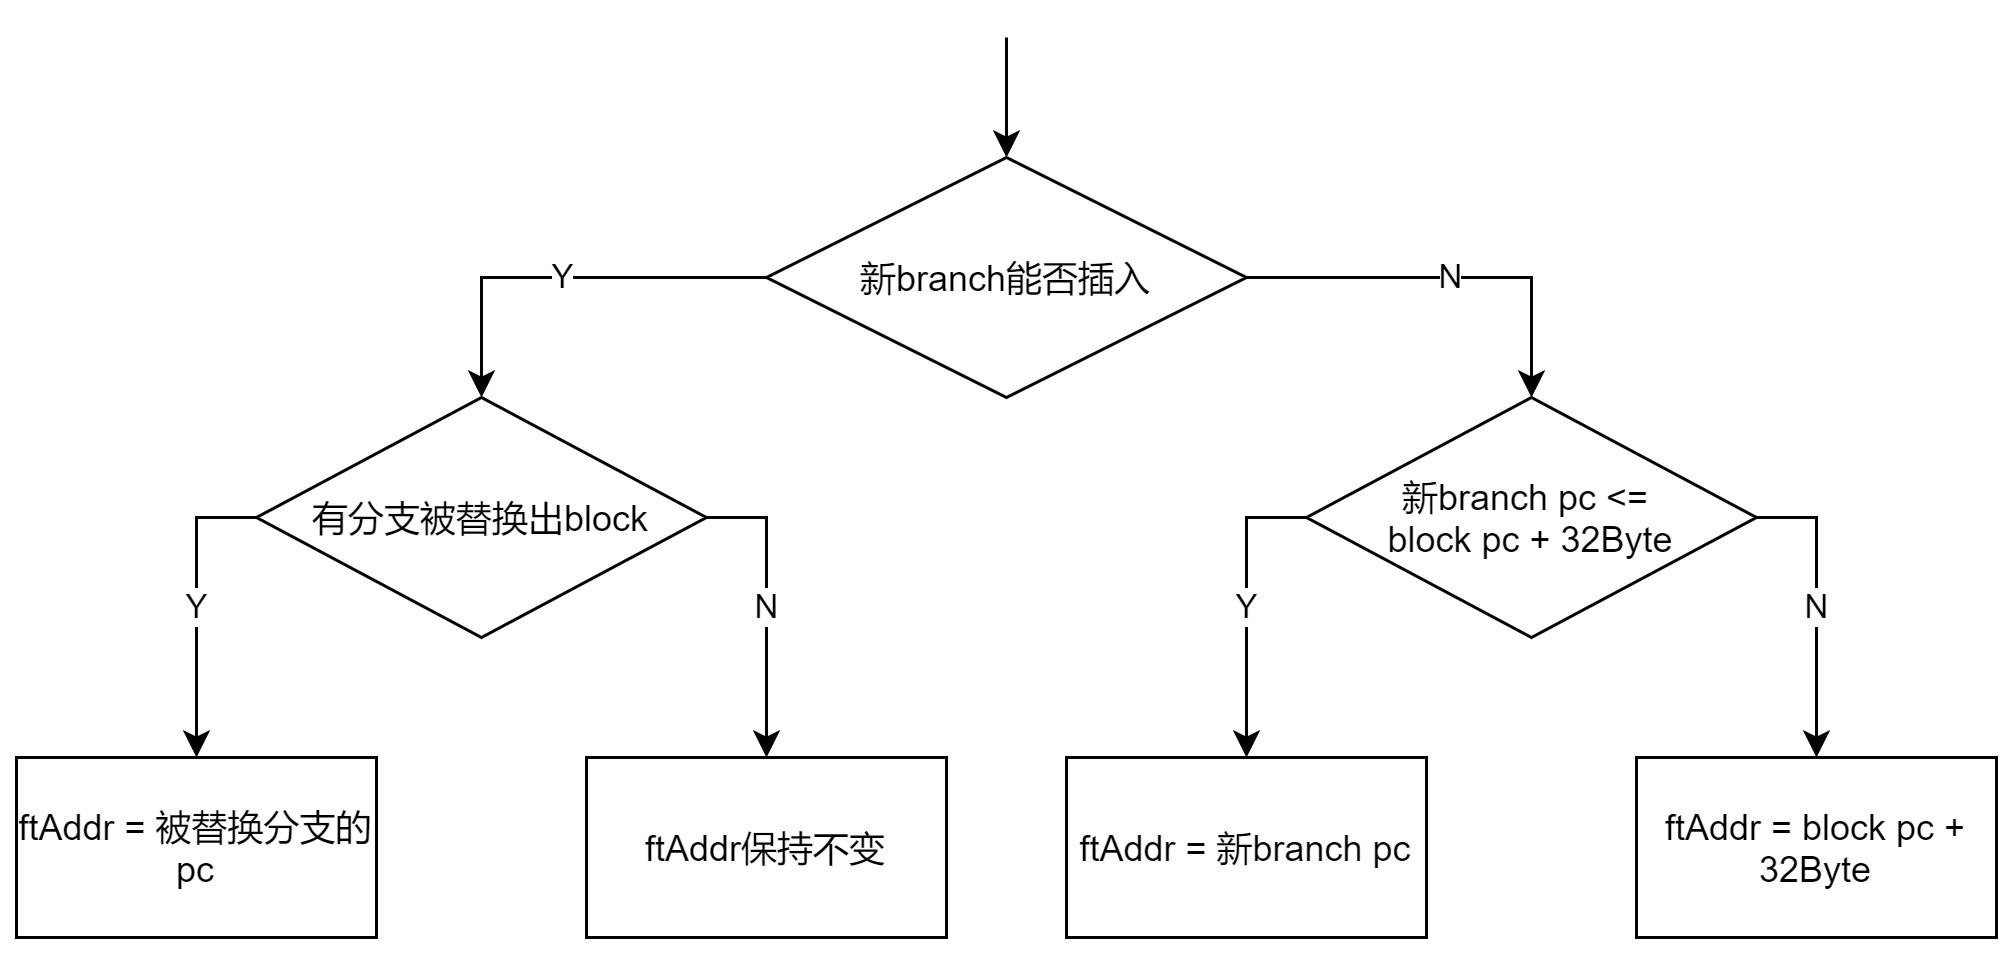
\includegraphics[width=1\textwidth]{ftb-manage.jpg}
	\caption{FTB更新时Fetch Block fallthrought address的变化,ftAddr表示fallthrough address}
	\label{fig:figure32}
\end{figure}

除了维护已有的Fetch Block,如果有新的block需要写入FTB,但是对应的way已满,则需要选择其中一个block替换出去,在雁栖湖架构的架构中BTB使用的是随机替换策略,在南湖架构中改为PLRU替换策略,并且使用的是用Chisel实现的通用替换策略模块,可以非常快速灵活的更改替换策略,在香山的各级缓存中使用的也是相同模块。

写入新的block时需要注意,如果这个block已经在FTB中存在,那么只需要更新其中的block即可,而不能够写入两个起始地址相同的block,这样会导致查找FTB时出现多路命中 (multiple hit) 的错误,这会影响到FTB中存储信息的正确性,从而影响分支预测的性能。因此,在添加或者替换block之前,首先需要确认这个block是否已经存在于FTB之中。最直观的方法就是查找一次FTB,就可以知道block是否已经存在,但是由于FTB是使用单口SRAM来存储主要数据的,一个周期内只能够读或者写,因此在添加或替换FTB时,首先需要阻塞分支预测流水线,因为分支预测也需要读FTB来获取分支相关的信息。然后花一个周期先读FTB,检查block是否已经在FTB中,如果在存在,在哪一个way中,如果不存在,则给它分配一个way,下一周期再写入FTB。这样一来,每次添加或替换FTB时,预测流水线都会堵塞2个时钟周期。这会导致预测效率的降低,为此做了以下两点优化,能够减少大部分指令提交时的FTB读需求:

\begin{enumerate}
	\item 在预测时会将当前预测的block是否在FTB中命中,以及哪一way命中的信息,作为FTB预测的meta信息传入FTQ中保存,而在这个block中的指令提交时,FTQ会将这个命中信号传回FTB,如果在预测时这个block就已经存在于FTB中了,那么在指令提交时这个block大概率仍然存在于FTB中,并且即使在这段时间内这个block被替换出FTB了,也依然不会出现multiple hit的情况。如果发现预测时这个block就已经在FTB中命中。只要直接将更新后的block写入预测时保存的那个way中即可,不用再查找一次FTB。当然如果没有命中,仍然还是要查找一次FTB。通常FTB的命中率很高,使用这种策略能够减少大量不必要的堵塞。
	\item 在试图更新block时,会检测block在这次提交中是否有新的分支,其中的信息是否有改动,如果这次提交没有给原有的block带来任何改动,那么就不用写入FTB,避免没有意义的写入。
\end{enumerate}

通过以上两点优化,可以极大减少由于更新导致的FTB读写,降低对分支预测流水线的影响。经过测试,在做这两点优化前,在更新时先查找FTB会极大的降低分支预测流水线的预测效率,而优化后对分支预测的影响几乎没有。

% 相关的性能验证放在第5章写吧

\section{本章小结}

本章以香山雁栖湖架构中的32Bytes对齐取指开始讨论,阐述了对齐取指和非对齐取指的优劣,并给出了为什么在南湖架构中要修改对齐取指这一策略。提出了一种FTB设计的详细实现方案,主要给出了FTB中用于存储Fetch Block的数据结构,并给出了在不同情况下Fetch Block更新时内部信息的管理策略,并提出了几种优化细节。最终将其应用在了香山处理器南湖架构的分支预测部件中。通过使用FTB替换雁栖湖架构的BTB,分支预测的整体预测宽度从16缩减到了2,减少了分支预测关键路径上的逻辑电路延迟。并且整体前端分支预测与取指的带宽没有太大的损失。
						
% !Mode:: "TeX:UTF-8"
\chapter{分支预测针对解耦前端的设计}

本章首先介绍前端解耦的含义,以及为什么需要对前端解耦,之后详细介绍解耦前端的设计中分支预测相关部分的设计,主要是介绍FTQ (Fetch Target Queue) 的功能和设计,FTQ作为连接分支预测部件和取指单元的关键部件,在承担保存取指请求功能的同时也承担了保存分支预测信息和管理后端指令提交信息的功能,通过FTQ能够让以Fetch Block为基本单位的分支预测部件和以单条分支为基本单位的后端流水线进行信息的交互,以实现必要的功能。

\section{香山雁栖湖架构耦合前端简介}

% 还没有介绍BPU的三级覆盖预测和分支历史管理机制
% 还没有介绍IUM
% 也没有讲各个部件SRAM尺寸的改变

在香山雁栖湖架构的设计中,而把分支预测和取指单元统称为流水线的前端。相对的以译码为边界,译码和译码之后的流水级统称为后端。而在雁栖湖架构的前端设计里,取指单元和分支预测的流水级是耦合在一起的,如图\ref{fig:figure41}所示。也就是说只有当分支预测和取指单元当前流水级都完成之后,才能够流向下一流水级,这会导致分支预测和指令缓存的访问互相阻塞。例如当访问指令缓存发现miss时,即使分支预测已经完成,也仍然需要停下来等待指令缓存从下级缓存中得到回填的数据;同样的当分支预测需要覆盖预测,冲刷流水线时,即使指令缓存已经准备好被访问了,由于流水线被冲刷,暂时没有新的访问请求,也只能够等待分支预测执行。将这种相互掣肘的耦合关系分开,可以将大量的前端气泡消除,即将分支预测流水线和取指流水线分离,中间由一个队列连接,这个队列就是FTQ (Fetch Target Queue)。

\begin{figure}[htb]
	\centering
	\setlength\tabcolsep{3pt}  % 同一行中的图片间隔
	\vspace{5pt} % 图片上部的空白,如果太小的话,图片顶部会与正文内容十分接近
	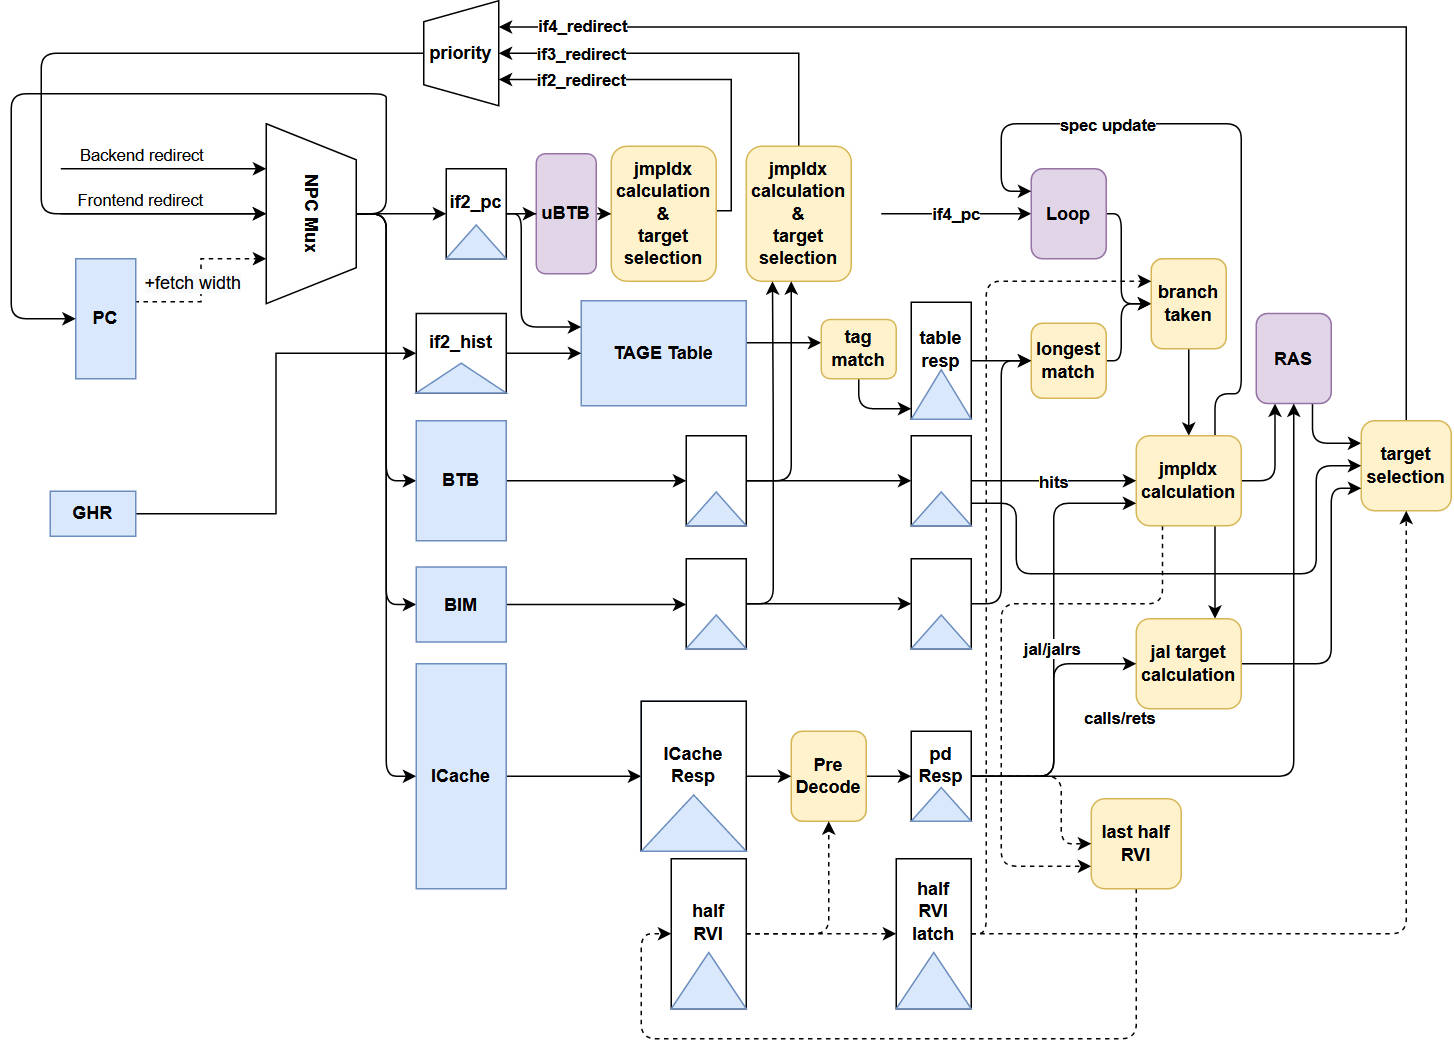
\includegraphics[width=1\textwidth]{yqh-IFU-BPU.jpg}
	\caption{香山处理器雁栖湖架构分支预测与取指架构图}
    \label{fig:figure41}
\end{figure}

\section{通过FTQ实现前端解耦}

通过将分支预测流水线和取指流水线解耦开,通过FTQ连接,如图\ref{fig:figure21}所示,就能够将分支预测和取指单元变成类似于生产者和消费者的关系:分支预测作为生产者,负责不断地预测当前pc下一拍的取指pc,而不用管指令缓存是否miss,只需要将相关的取指请求放入FTQ之中。而取指单元作为消费者,负责不断地从FTQ中顺序取出取指的请求,访问指令缓存得到指令码,将它传给后端。由于在指令缓存miss时,分支预测仍旧会不断地往FTQ中送入取指请求,因此当分支预测冲刷流水线时,取指单元也不用等待,可以继续取出FTQ中之前存储的取指请求,继续访问指令缓存。这样一来就能够减少前端很多不必要的气泡,前端的供指效率能够得到提高,这也会对整体架构的性能有一定的正面影响。

FTQ同时连接着分支预测、取指单元和后端执行单元,除了用于将分支预测和取指单元解耦,还负责记录所有在流水线中执行指令的状态,并保存分支预测信息和指令预译码信息。并负责接收从后端和取指单元传来的redirect信息,包含分支误预测和指令replay请求,并给分支预测和取指单元发送恢复信号和必要信息。FTQ的每个项代表了一个Fetch Block,当FTQ中的一个block里所有的有效指令都被提交后,FTQ会给分支预测发送commit信息,用于训练分支预测器。

\subsection{FTQ中的存储结构}

FTQ本质上是一个队列,其中有4个指针,分别代表所有指令在流水线中的不同进度。

\begin{enumerate}
	\item bpuPtr:类似队尾指针,当分支预测产生新的取指请求时从这个指针指向的位置入队
	\item ifuPtr:指向最近一次发送给取指单元的block
	\item ifuwbPtr:指向最近一次从取指单元写回预译码信息的block
	\item commPtr:类似队头指针,指向最近一次被提交的block
\end{enumerate}

FTQ是一个循环队列,其中使用的指针都是FtqPtr类的实例,设计参考了《超标量处理器》中的设计\cite{superscala}。每个指针有flag和value 2个值,其中value代表这个指针指向的是队列中第几个元素,而flag代表的是这个指针在哪一次遍历,如图\ref{fig:figure42}所示,图\ref{fig:figure42}(a)中tail指向第4个元素,head指向第2个元素,tail和head都在同一次遍历中,flag都为0,灰色代表了队列中有效的项。而图\ref{fig:figure42}(b)中继续入队出队后,head指向了3,而tail已经完成了一次遍历,再次从0开始向后遍历到了1,此时head和tail不在同一次遍历中,head的flag为0,而tail的flag为1,此时队列中的有效项不在head和tail之间,而是相反的。图\ref{fig:figure42}(c)中当head也完成了一次遍历,回到0时,此时head和tail的flag再次变为相同,都为1,有效项也变回了head和tail之间的项。使用这种方法,就可以很好的解决循环队列中不知道head和tail在哪一轮遍历中的问题。除了FTQ以外,这种数据结构在香山的其他部件中也有广泛的应用。

\begin{figure}[htb]
	\centering
	\setlength\tabcolsep{3pt}  % 同一行中的图片间隔
	\vspace{5pt} % 图片上部的空白,如果太小的话,图片顶部会与正文内容十分接近
	\begin{tabular}{ccc}
		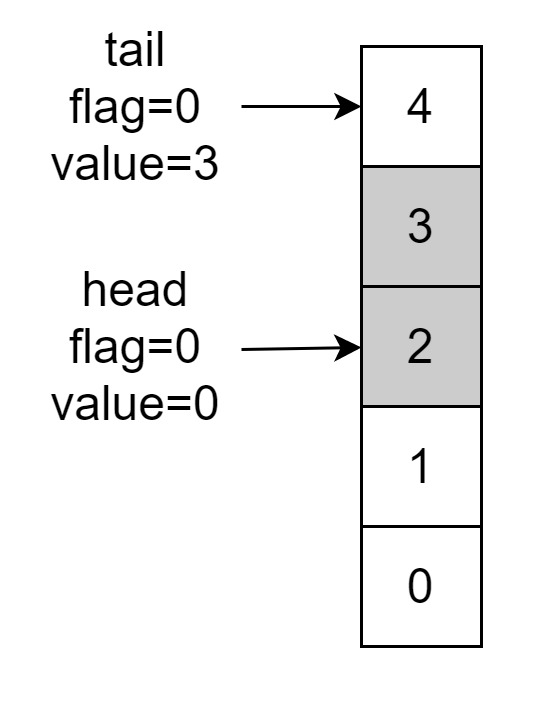
\includegraphics[width=0.23\textwidth]{queue_ptr_a.jpg} &
		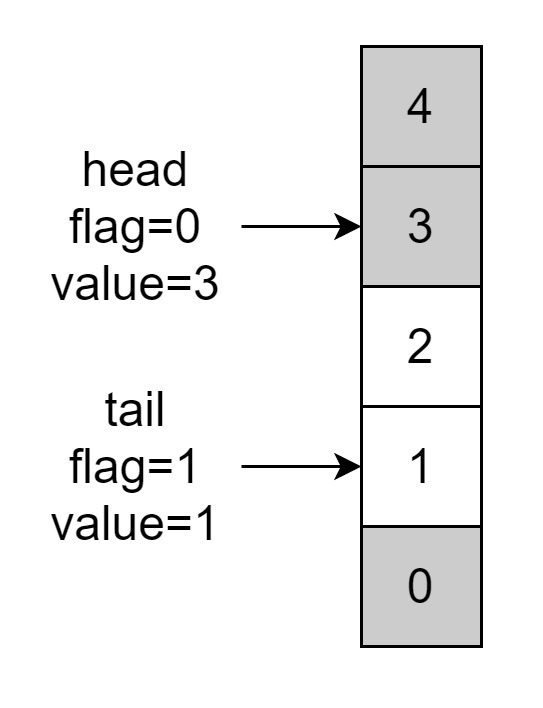
\includegraphics[width=0.23\textwidth]{queue_ptr_b.jpg} &
		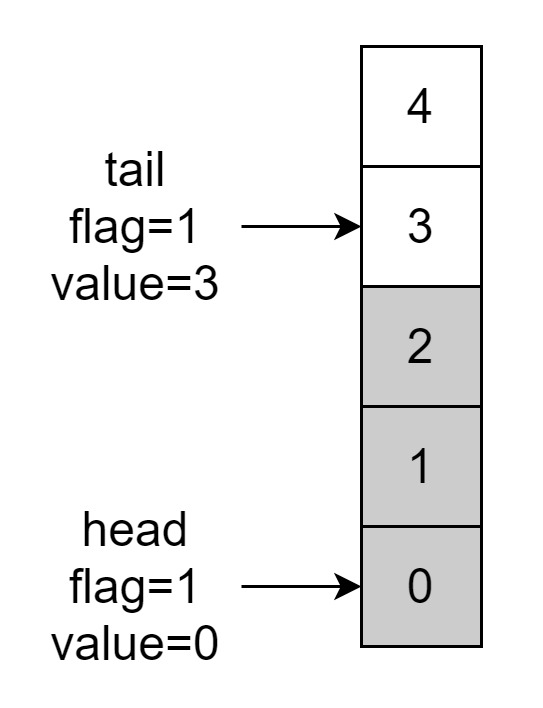
\includegraphics[width=0.23\textwidth]{queue_ptr_c.jpg} \\
		(a) & (b) & (c) \\[1ex]
	\end{tabular}
	\caption{通过flag来表示head和tail是否在同一轮遍历中}
	\label{fig:figure42}
\end{figure}

在FTQ中的表项需要存储的信息分为几类,分别存在不同的寄存器堆中,大致分为以下几类:

\begin{itemize}
	\item pc相关信息。主要存储block的起始地址,以及一些其他的信号位。在分支预测有新的取指请求,以及分支预测redirect时写入。
	\item redirect分支预测重定向相关信息。分支预测在redirect恢复时需要的一些信息,例如RAS栈顶元素和栈顶指针,全局历史指针等。在分支预测最后一个流水级fire时写入
	\item 分支预测meta信息。用于保存所有预测器在预测时产生的meta信息,是一个很长的Unsigned Int,将所有的meta信息都转成Unsigned Int拼接起来,拼接和拆分由Composer组件负责。在分支预测最后一个流水级fire时写入
	\item FTB表项。存放从分支预测传来的FTB表项。在分支预测最后一个流水级fire时写入,用于判断是否出现false\_hit,以及在指令提交时判断表项有无改变,产生新的表项。
	\item 预译码信息。用来存储取指单元写回的预译码信息,用于在指令提交时生成新的FTB表项。
\end{itemize}

FTQ中有一个状态队列commitStateQueue,用来表示每个表项代表的Fetch Block中所有指令的状态,有invalid,valid,commited三个状态。当一个block中只有invalid和commited时,代表这个block中所有的有效指令都已经提交了,这时就可以以整个block为单位,给分支预测发送更新信号。当有redirect信号时,这个队列也要进行恢复。

此外还有一个表示FTB hit状态的队列entry\_hit\_status,用来表示Fetch Block在FTB中的hit状态,有not\_hit,hit和false\_hit三个状态。其中false\_hit状态表示的是在查找FTB时hit了,但是Fetch Block中有分支指令的信息与预译码不符,例如在block中的offset不同,分支指令的类型错误等情况。出现这种情况原因是因为在FTB中存储的tag不是完整的tag,当程序达到了一定的大小,就有可能出现别名的情况,即两个不同的Fetch Block的tag相同,但是其中的分支信息完全不同。但是这种情况比较少出现,对性能影响有限,而不使用完整的tag可以一定程度上减少SRAM的大小。

在FTQ入队时每个表项都只会是hit或者not\_hit的状态,但是在取指单元写回预译码信息后,FTQ会根据预译码信息将部分hit信号修改为false\_hit。

保存FTB hit的状态可以用于分支历史的更新,以及控制FTQ发送更新信息给FTB的时机。由于在第三章中提到,FTB在预测时没有hit,那么更新前就要先查找一遍FTB,然后再写入,需要2个周期,但是有可能连续几个周期都有block被提交了,因此FTQ要根据FTB是否hit,来决定什么时候给FTB发送更新请求。

\subsection{FTQ的行为逻辑}

当分支预测S1完成后,就会将刚才预测的pc传给FTQ,如果FTQ未满,则会将其入队,同时bpuPtr递增。如果队满了则会阻塞分支预测的流水线,而由于FTQ满基本上意味着前端供指充足,因此这种阻塞不会影响处理器的整体性能。FTQ中有bypass逻辑,如果取指单元已经准备好访问指令缓存,那么下一周期就可以将这个取指请求送往取指单元访问指令缓存。否则则储存在FTQ中。

由于在S1预测时还没有得到FTB等其他预测器的返回结果,因此S1时入队的FTQ项中有效的只有pc相关的信息。S1入队后FTQ会返回指向新入队表项的指针,在分支预测全部结束之后,会将剩余的信息补充到表项中。

由于分支预测采用的是覆盖预测机制,即当后面的流水级中更准确的预测器预测结果与前面的流水级不同时,以后面的流水级为准,并且冲刷流水线,恢复之前错误的取指请求。因此FTQ在分支预测冲刷流水线时,相应的要将bpuPtr,ifuPtr和ifuwbPtr都恢复到正确的位置。同时由于这时候可能已经有错误的请求发往取指单元了,因此也要给取指单元发恢复请求。

在取指请求发给取指单元,取指单元取回指令完成预译码后,要将预译码的信息传回给FTQ储存起来,同时要判断一些简单的误预测,例如一些jump指令被预测为不跳转。同时还会修改commitStateQueue的状态,将对应的项改为valid,代表指令已经送去后端流水线执行,但是还没有提交。

FTQ也要将分支预测的结果传给后端执行单元,在分支指令执行后要再次和预测结果比较,最终确定分支指令有没有误预测。

取指单元和后端执行单元都有可能发现分支误预测,误预测时需要给FTQ发送redirect分支预测重定向信号,假如两者同时发现误预测,由于正在执行单元的分支指令指令序比在取指单元的分支指令早,因此以后端的redirect信号为优先。

FTQ收到redirect信号之后,会拿到取指单元或后端发回的出现了误预测指令的FTQ表项的指针,根据这个指针将相关的数据从FTQ中取出,进行处理后向分支预测发送redirect信号,恢复分支预测器以及分支历史。如果redirect来自后端,那么也要给取指单元发redirect信号,因为取指单元也需要恢复错误的取指。同时需要恢复bpuPtr,ifuPtr和ifuwbPtr到redirect发回的指针加1的位置,因为这条误预测的指令以及之前的指令仍然是要提交的。同时需要将误预测指令所在的Fetch Block中所有在这条指令之后的指令状态都置为invalid。

当有指令提交时,FTQ需要将对应的指令的状态改为commited,当一个block中的所有指令状态是invalid或commited,并且其中有跳转的指令,或者曾在FTB中命中,那么block就可以向分支预测提交了。提交时会从FTQ中取出对应的预译码信息,meta信息等,送往分支预测用于更新预测器的训练数据。

% FTQ会接收BPU s2和s3的信号,当分支预测部分有redirect时,FTQ中也要将指针恢复到正确的位置

% 每次有取指请求入队时,FTQ需要给分支预测返回新入队的项的bpuPtr,在分支预测redirect时需要用这个指针进行恢复。

% 取指请求在分支预测S1 fire和S2,S3 redirect的时候发送给FTQ

% FTQ中的存储结构(或者说FTQ表项中的组成部分)主要有:

% update\_target
% cfiIndex\_vec
% mispredict\_vec
% pred\_stage

% entry\_fetch\_status。用来表示FTQ项对应的取指状态

% entry\_hit\_status。用来表示FTQ项在FTB的hit状态,有not\_hit,hit和false\_hit。

% 当分支预测s2和s3需要redirect时,FTQ要负责把bpuPtr和ifuPtr都移动到正确的位置。同时把redirect信号发给IFU,IFU对之前的错误的取指进行恢复

% FTQ有bypass操作,如果上一拍BPUfire,且ifuPtr等于当前的bpuPtr,就直接将最新的取指请求发给IFU

% FTQ还要接收从IFU写回的信息,在取指请求发给IFU,IFU取回指令码,并预译码之后,会将预译码信息传回FTQ保存起来,同时IFU还会检测是否有明显的误预测,如果有也会发给FTQ,由FTQ给分支预测发送误预测恢复信号。并将commitStateQueue有效的指令状态修改为valid

% 写回后还会和之前保存的FTB entry进行判断,有没有false\_hit,当FTB hit,但是预译码结果和FTB entry中的结果不一致时,则认为是出现了false\_hit的情况,具体可能有是分支不是分支,是跳转不是跳转,以及跳转目标地址的offset不同

% FTQ还要将指令信息传给后端,由后端执行时再做一次判断,决定是否误预测

% 当后端发现误预测指令时,后端回发回误预测信号和误预测指令所在block的FtqPtr,FTQ根据这个指针去读取ftq\_redirect\_sram和ftb\_entry\_mem中的数据,将这些数据进行处理后发送回分支预测,并更新分支历史

% IFU发的redirect也和后端的处理方式类似

% RedirectGen。接收后端发来的信息,生成redirect信号

% 恢复指针和state queue。在有误预测时,需要恢复FTQ的指针和状态队列,redirect的来源有后端和IFU,同时发redirect时以后端的优先,在redirect发生时,无论是后端还是IFU,都会发回发生redirect的block在FTQ中对应的指针,需要将bpuPtr,ifuPtr,ifuwbPtr都恢复到redirect 指针加1的位置,因为误预测的指令所在的block也是需要提交的。同时需要将block中误预测指令之后的所有指令的状态都置为invalid。

% 后端发redirect时,FTQ不光要给分支预测发redirect,也要给IFU发

% 每当有指令提交时,FTQ需要将对应指令的状态修改为commited

% 当一个block中的所有指令状态是invalid或commited,并且其中有跳转的指令,或者曾在FTB中命中,那么block就可以向分支预测提交了。提交时会把ftq\_pc\_mem,ftq\_pd\_mem,ftq\_redirect\_sram,ftq\_meta\_1r\_sram,ftb\_entry\_mem中commPtr中对应的数据都取出来,用于生成传给分支预测的分支预测训练数据。

% FTQ会控制发送commit的频率,如果某次更新FTB需要先查找FTB再写入,那么FTQ就会将之后的commit请求延后,等到FTB准备好下一次更新时再发送。

% FTB中表项的更新逻辑由FtbEntryGen中实现

% FTQ还有一些支持指令预取的逻辑




% 雁栖湖架构的分支历史是按照一个packet 1 bit的,南湖架构是每条分支1 bit

\section{本章小结}

本章首先介绍了雁栖湖架构设计中分支预测与取指单元耦合带来的影响,为什么在南湖架构中决定解耦前端,以此引出设计FTQ这个模块的意义。之后介绍了FTQ是如何时前端解耦的,基本的功能。再进一步介绍FTQ中存储的分支预测信息和指令信息的组织结构,最后再详细介绍了FTQ和分支预测、取指单元、后端执行单元的交互逻辑。
						
% % !Mode:: "TeX:UTF-8"
\chapter{分支预测性能优化方向探索}
本章主要介绍
\section{小节名称}

\section{本章小结}

						
% !Mode:: "TeX:UTF-8"
\chapter{行为级仿真,时序分析及性能验证}

通过前面几章,详细描述了整个分支预测框架的设计细节,以及南湖架构相对于雁栖湖架构做出的改进。本章主要介绍所有的工作实现后,如何从多个方面来评估设计带来的提升,首先介绍香山使用的评估环境,由于南湖架构设计还没有正式的流片成功,且FPGA也还未成功运行,因此目前仍然是使用在服务器上用软件进行行为级仿真的方式来测试设计的正确性和性能。这种方式相比于最终的流片结果测试数据会有一定误差,但是通过和雁栖湖架构代码使用相同行为级仿真的测试方法测出的结果来比较性能的提升依然是有一定说服力的。然后介绍行业内认可度比较高的,测试整体性能的评估程序Coremark和SPEC CPU 2006,最后介绍与整体性能或分支预测性能相关的一些评估指标,并解释选择这些指标的原因。之后通过统计对比香山雁栖湖架构和香山南湖架构的实验结果,体现本文设计的有效性和带来的提升。

\section{开发工具与实验平台}

\subsection{Chisel}

Chisel (Constructing Hardware In a Scala Embedded Language) 是加州大学伯克利分校开发的一种开源硬件构造语言,它是一个建构在Scala语言\cite{scala}之上的领域专用语言 (DSL, Domain-Specific Language),不同于硬件设计领域传统的Verilog语言,Chisel建立在Scala这门高级编程语言之上,香山开发之所以选择使用Chisel语言,是因为Chisel在具有更加高级的语言特性的同时又没有丢失底层电路设计的细节,能够使用大量高级语言才有的特性,比如面向对象编程和函数式编程的思想,能够从更高的抽象程度来描述硬件电路,实现更多Verilog难以完成的功能,极大的提高使用者的开发效率。

\subsection{差分测试框架}

在开发过程中,由于硬件电路非常复杂且难以调试,不同于软件开发有各种各样完善的调试工具,可以下断点追函数调用等,且由于仿真速度的限制,运行一次测试的时间也比普通的软件开发慢很多。因此香山团队开发了一套差分测试框架,如图\ref{fig:figure64}所示, 即使用一个认为是实现正确的指令集模拟器NEMU\cite{nemu},和硬件设计的仿真同时运行,并以NEMU为参考,在指令提交时比较两者的寄存器堆中的值是否相同,来判断硬件设计运行时有没有出现指令执行结果错误的情况,当发现比对结果不同时,立即中断仿真,并输出相关的处理器内部状态,以此来提高发现和定位问题的效率。当然由于分支预测的特殊性,一些只影响分支预测准确率的功能实现错误时,例如分支历史更新逻辑有问题,这种情况下只会影响性能,程序依然能够正确的执行完毕。因此这种错误使用差分框架难以发现。

\begin{figure}[htb]
	\centering
	\setlength\tabcolsep{3pt}  % 同一行中的图片间隔
	\vspace{5pt} % 图片上部的空白,如果太小的话,图片顶部会与正文内容十分接近
	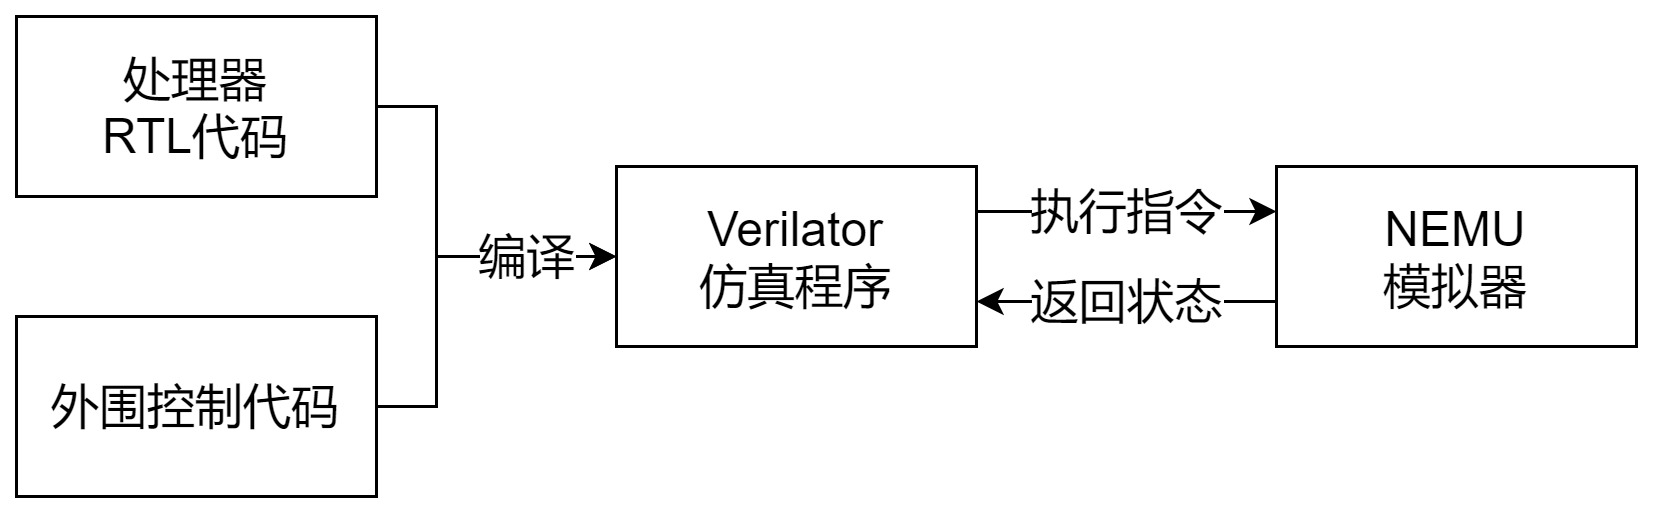
\includegraphics[width=1\textwidth]{diff.jpg}
	\caption{差分测试框架,NEMU和仿真程序同时运行,比较运行结果}
	\label{fig:figure64}
\end{figure}

\subsection{Verilator}

Verilator\cite{verilator}是一款开源免费的Verilog/System Verilog仿真器,可用于将Verilog代码转换成C++代码,在服务器上通过运行软件程序对硬件设计进行行为级仿真验证。相比于类似的另一种仿真工具VCS\cite{vcs},由于Verilator仿真的电路只有0和1两个状态,不同于VCS有0、1、X、Z四个状态,因此在运行处理器这种大型的电路仿真时,Verilator仿真运行的速度会比VCS更快。但是毕竟处理器整体的RTL设计过于复杂,因此Verilator的仿真速度在跑SPEC CPU 2006这类大型测试程序时依然是一个瓶颈。相比于差分测试框架中纯软件的指令集模拟器NEMU来说,运行速度差了好几个数量级。

\subsection{Design Compiler}

Design Compiler是Synopsys公司开发的用于对电路进行综合以及静态时序分析 (STA, Static Timing Analysis)的核心工具,能够添加各种设计约束,将电路设计的RTL代码转换为基于工艺库的门级网表,并从速度、面积和功耗各方面来优化和评估电路设计,是RTL代码时序调优过程中一个重要的工具。

\section{验证环境与评估指标}

\subsection{验证环境}

硬件部分CPU使用的是AMD EPYC 7742 128核,操作系统是Ubuntu 20.04.3 LTS。在服务器上对设计进行行为级仿真来进行验证与评估,首先通过脚本将Chisel编写的RTL代码编译成功能相同的Verilog代码,然后再用Verilator将其转变为仿真用的可执行文件,在电脑上运行行为级仿真,模拟电路运行时的状态。

通过差分测试框架,NEMU会和需要仿真的电路同时运行,由于NEMU执行指令的速度比仿真程序快了好几个数量级,且占用资源极少,因此并不会对仿真测试运行的时间带来太大的影响,且可以随时监控电路仿真有没有出现指令执行错误的情况,及时中断仿真并报告出错现场。

在开发过程中,会使用的测试程序有很多,通常一些小的改动和简单测试,会运行Coremark,这是由EEMBC发布的测试处理器核心性能的一项基准测试程序,程序使用C语言写成,主要功能包含如下四类运算法则:

\begin{enumerate}
	\item 数学矩阵操作(普通矩阵运算)
	\item 列举(寻找并排序)
	\item 状态机(用来确定输入流中是否包含有效数字)
	\item CRC(循环冗余校验)
\end{enumerate}

Coremark程序比较小,运行一次需要的时间很短,但是为了能够让处理器充分运行起来,例如给分支预测一些训练的时间,因此在跑Coremark时通常都会连续执行很多次迭代,例如迭代运行100次。通过运行Coremark,在初步的开发时,一些很容易触发的,比较明显的bug就能够很快的找到。并且由于运行一次的时间很短,因此修改bug时可以快速迭代。

此外在需要更多的测试程序,想要测试更多复杂的情况时,通常会通过运行SPEC CPU 2006\cite{spec-2006}来测试电路性能。SPEC CPU 2006是SPEC (Standard Performance Evaluation Corporation) 组织推出的CPU系统评估软件,是业内比较权威的性能参考指标,SPEC CPU 2006中包含有SPECint 2006和SPECfp 2006两个基准,SPECint 2006中包含12个不同的基准测试,SPECfp 2006中包含19种不同的基准测试。SPEC CPU 2006和SPEC CPU 2017也是香山发布时公开的最主要的性能数据,大量的处理器相关研究都会以这两个测试的得分来评估性能。

除此之外还有其他的测试程序,例如Dhrystone\cite{dhrystone}、SPEC CPU 2017,以及一些简单小程序的集合Microbench。针对某些特定的模块,也会有针对特定功能的单元测试程序。

% 找耀阳师兄要引用

值得一提的是由于香山整个项目的设计非常复杂,因此在使用Verilator进行行为级仿真时速度非常慢,在运行Coremark这类程序时所花费的时间还可以承受,但是当需要运行SPEC测试时,所需要花费的时间就要按月计算。香山团队开发了一套基于checkpoint的测试方法。其主要思路在于通过神经网络训练,找到一个程序中最具有代表性的片段,并给出各自的权值,能够保证运行完这些片段之后将其对应的性能数据乘以权值的和尽可能接近完整的测试程序运行结果。这样的话就不用运行完整的测试程序,只运行一些程序片段即可。且因为一个程序被切分为许多片段,因此可以通过并行运行这些片段来进一步缩短测试运行的时间。

由于有一个运行速度极快的指令集模拟器NEMU,因此可以先使用NEMU来训练切片,验证片段的准确性,然后再使用Verilator仿真运行这些程序片段,真正验证物理设计电路的性能。

因为checkpoint在恢复时只能够恢复内存和寄存器,像FTB这类SRAM无法完全恢复,所以在真正的测试片段运行前,需要运行测试片段前的一小部分程序,为整个流水线做warmup,经过一段时间的训练后再开始运行正式的测试片段。通过这种技术,可以在几周内就得到一次完整的SPEC测试数据,极大提升了迭代效率。

由于运行一次完整的SPEC CPU 2006测试,即使使用了checkpoint技术,也需要几周的时间。因此为了更快的得到测试的性能结果,本文的性能评估一节中,只选取了SPEC CPU 2006的部分有代表性的测试点进行测试。

通过在代码中添加各种各样的性能计数器。在测试程序执行完毕后,可以通过查看性能计数器的结果,来判断分支预测部分的工作情况,并通过跟香山雁栖湖架构的相关数据进行比对,来验证南湖架构设计的性能提升。

在整体架构的RTL设计完成,并且通过测试后,再使用Design Compiler对整体架构进行静态时序分析,评估设计中各条逻辑电路的延迟,是否满足目标频率的约束条件,然后从其中找到时序违例的电路,对其功能和实现进行分析,优化调整之后再次迭代,直到最终所有的电路都能够满足目标时序的要求。以最终的时序评估结果作为流片时芯片主频的参考。

\subsection{验证评估指标}

本文的评估指标有:

\begin{enumerate}
	\item IPC (Instructions Per Cycle)。即每周期有多少条指令提交,用总的指令数除以程序运行的总周期数计算得到。这是评估整个处理器架构性能的关键指标,IPC越高,说明单位时间内处理器能够执行的指令越多,性能越好,且IPC以周期数为衡量指标,可以很好的排除频率的影响。
	\item 分支预测准确率。即用预测正确的分支数量除以总分支数量,即可得到分支预测准确率,相反的,用预测错误的分支数量除以总分支数量,得到的就是分支误预测率,分支预测准确率加分支误预测率等于1。分支预测准确率可以比较直观的看出分支预测的性能。在现代处理器的分支预测设计下,基本上预测准确率能够达到90\%以上。
	\item MPKI (Misprediction Per Kilo Instructions)。代表在整个测试程序中每1000条指令中误预测指令的数量。也是衡量分支预测性能的一个重要指标。与分支预测准确率不同的是,MPKI除了考虑了分支指令以外,将所有的指令都纳入了考虑的范围内。通常情况下希望MPKI越低越好,但是导致MPKI低的原因不只有分支预测准确率高,一个分支指令数量在总指令中占比比较低的程序也有可能达到很低的MPKI,即使它的预测准确率较低。使用MPKI评估分支预测性能的原因是现在分支预测在很多情况下的准确率都已经非常高,一些应用甚至准确率能够达到99\%,这种情况下再对比分支预测准确率的差距变得不够明显。此外使用MPKI也能够更直观的看出误预测分支指令在整个程序中的占比,更容易评估误预测带来的penalty。
	\item FTB命中率。这是用于评估FTB的一个主要指标,在南湖架构的前端设计中,主要靠FTB来识别并给出分支指令的相关信息,如果FTB没有命中,分支预测就无从谈起,因此FTB的命中率也是影响分支预测准确率的一个重大因素。
	% \item 前端气泡数量?
	\item 频率。通过计算IPC,能够得知处理器整体架构每周期有多少条指令提交,除了提升IPC能够提高处理器的性能之外,提升频率也是一个重要的途径。频率越高,代表处理器每周期的时间越短,相同时间内包含更多周期,因此在相同IPC的情况下,频率越高,单位时间内处理器能够执行的指令数量也越多,总体性能越高。达到更高的频率也是南湖架构相对于雁栖湖架构的一个主要提升方向。
\end{enumerate}

\section{评估结果分析}

本节将根据上一节提出的评估指标,来对SPEC CPU 2006的部分测试成果进行分析。主要用于对比的是香山处理器雁栖湖架构和南湖架构,因为香山南湖架构主要是在雁栖湖架构的基础上进行迭代优化,希望能够进一步的提升性能。

图\ref{fig:figure61}是运行占80\%权重的SPEC CPU 2006部分测试程序片段后,雁栖湖架构和南湖架构的IPC数据对比,可以看出南湖架构相比于雁栖湖架构的性能,大部分的程序IPC都有了提升,总体的IPC平均提升了30.96\%。当然IPC提升的原因有很多,南湖架构相比于雁栖湖架构的改进也不只是重构分支预测和解耦前端。因此IPC并不能够直观的反应分支预测单元性能的提升,但是解耦前端消除的气泡带来的性能提升依然占其中一部分比例。而由于两个版本架构解耦前后的前端差距过大,因此没有办法很好的控制变量,精准的测试出解耦带来的性能提升。

% 9.32 -18.4 17.6 67.05 28.57 58.57 51.19

\begin{figure}[H]
	\centering
	\setlength\tabcolsep{3pt}  % 同一行中的图片间隔
	\vspace{5pt} % 图片上部的空白,如果太小的话,图片顶部会与正文内容十分接近
	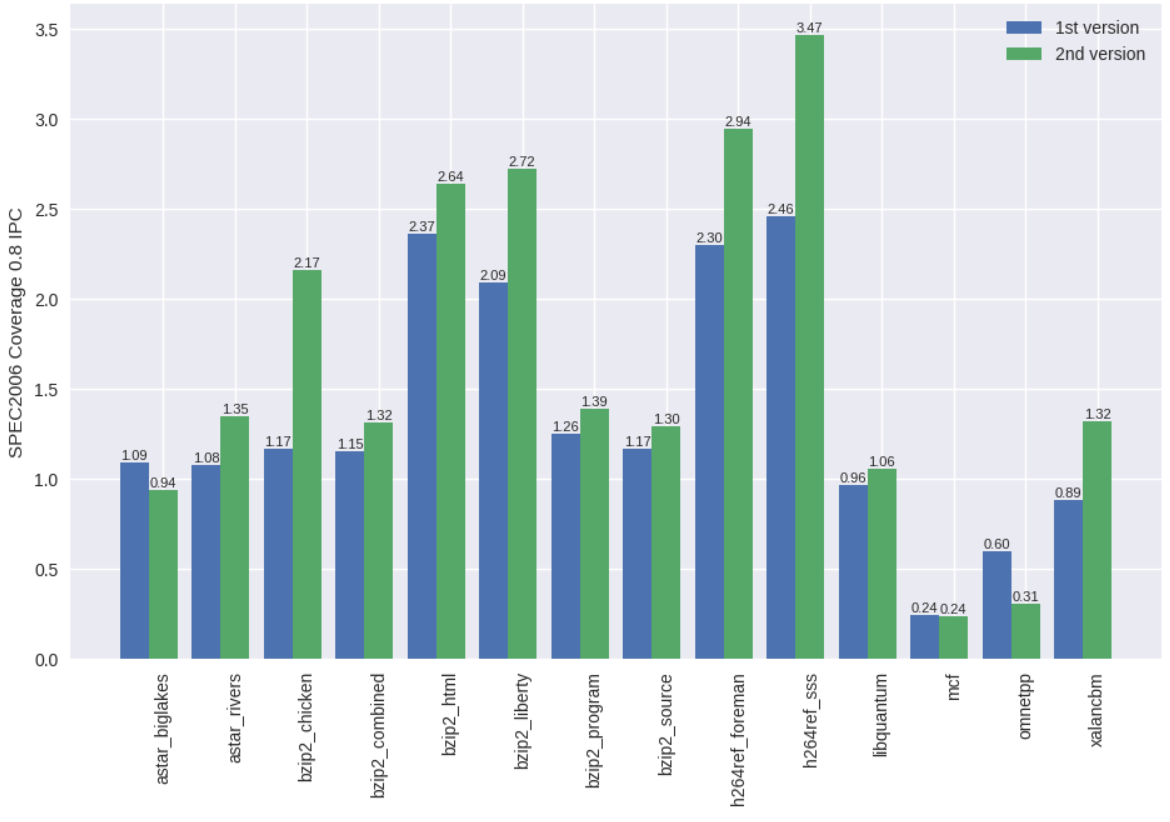
\includegraphics[width=0.9\textwidth]{ipc.png}
	\caption{SPEC CPU 2006 coverage 0.8 部分检查点IPC对比}
	\label{fig:figure61}
\end{figure}

图\ref{fig:figure64}和图\ref{fig:figure62}分别是运行占80\%权重的SPEC CPU 2006部分测试程序片段后,雁栖湖架构和南湖架构的分支预测准确率和MPKI对比。可以看出相比于雁栖湖架构设计,南湖架构设计的平均分支预测准确率提高了0.6\%,平均MPKI降低了1.13。分支预测性能变化的主要因素,主要有在南湖架构中使用了更加准确的单条指令的分支历史,并且增加了FTB使用的SRAM的容量,这些改动会对分支预测准确率有一定的正面影响,但是为了优化逻辑电路的延时,提高最终的频率,分支预测依然在很多方面做了性能上的妥协,例如减少了TAGE预测表的数量等细节上的处理,各种因素综合,得到了最终的性能变化。

\begin{figure}[htb]
	\centering
	\setlength\tabcolsep{3pt}  % 同一行中的图片间隔
	\vspace{5pt} % 图片上部的空白,如果太小的话,图片顶部会与正文内容十分接近
	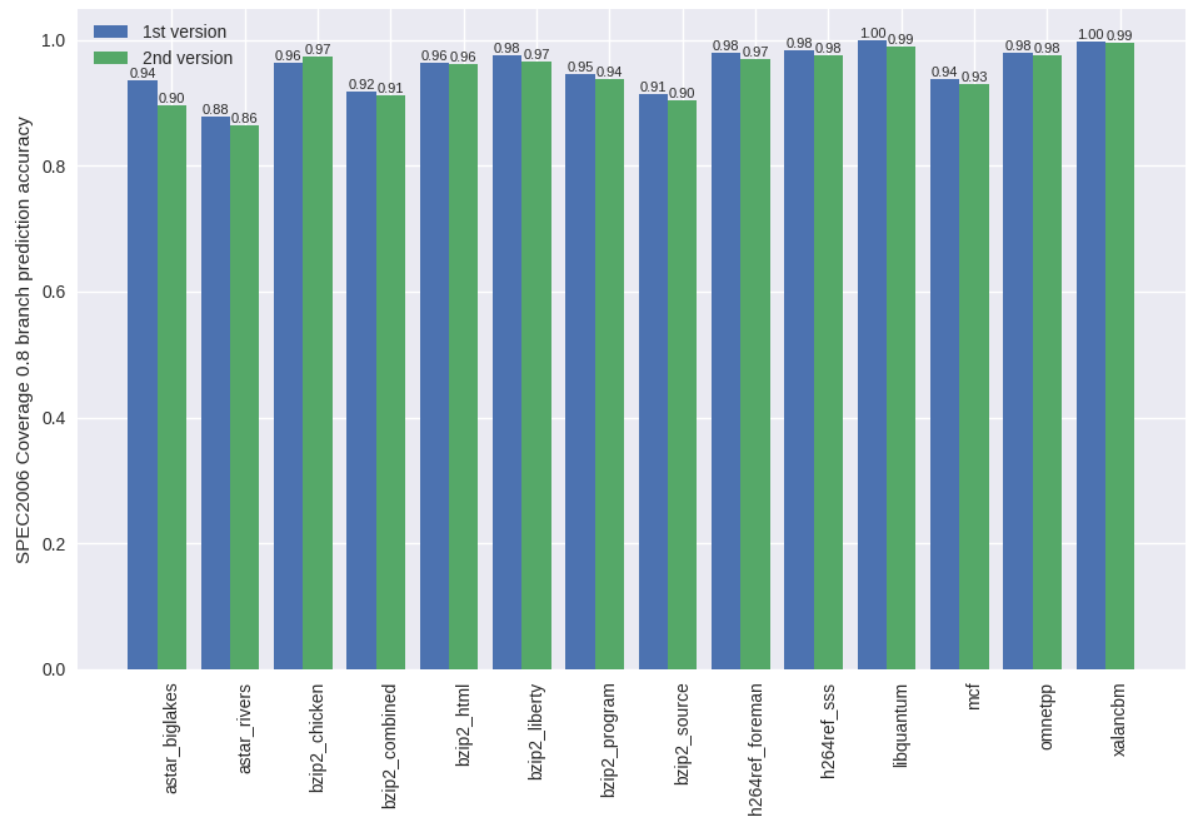
\includegraphics[width=0.9\textwidth]{accuracy.png}
	\caption{SPEC CPU 2006 coverage 0.8 部分检查点分支预测准确率对比}
	\label{fig:figure64}
\end{figure}

% 13.05 -39.61 40.68 86.36 20.68 -1.6 


\begin{figure}[H]
	\centering
	\setlength\tabcolsep{3pt}  % 同一行中的图片间隔
	\vspace{5pt} % 图片上部的空白,如果太小的话,图片顶部会与正文内容十分接近
	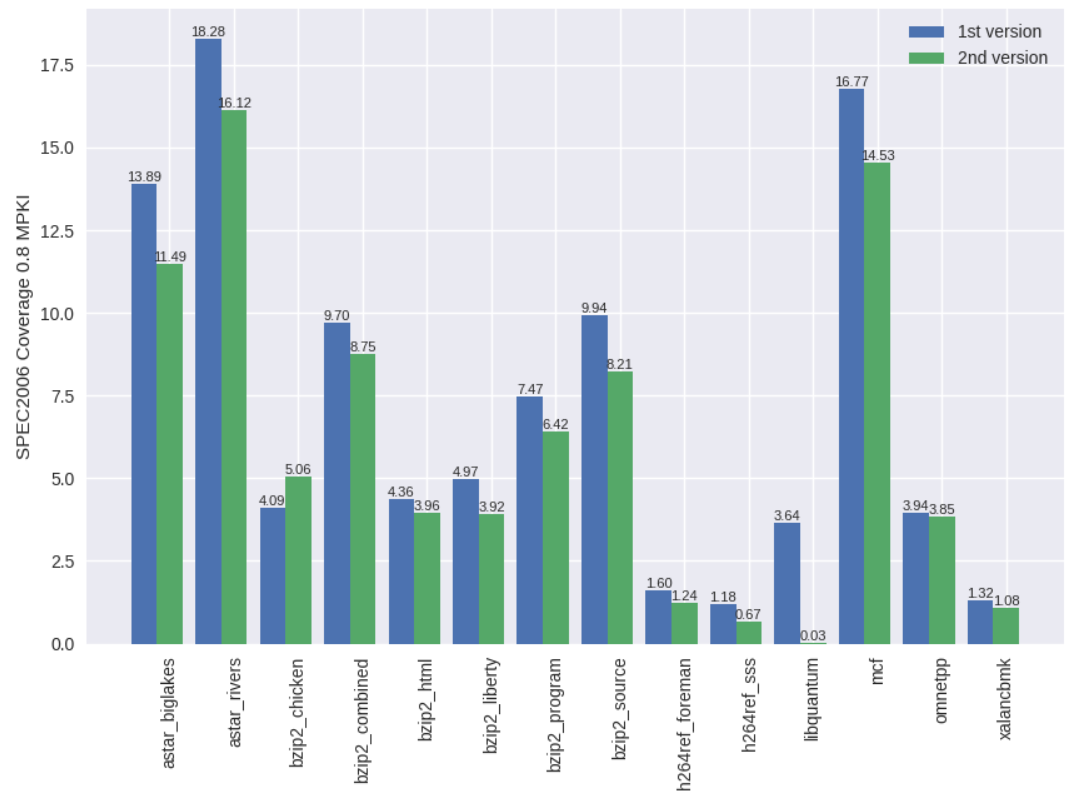
\includegraphics[width=0.9\textwidth]{mpki.png}
	\caption{SPEC CPU 2006 coverage 0.8 部分检查点MPKI对比}
	\label{fig:figure62}
\end{figure}

图\ref{fig:figure63}是在SRAM大小相同的情况下,运行占80\%权重的SPEC CPU 2006部分测试程序片段后,雁栖湖架构和南湖架构BTB和FTB的命中率对比,可以看出相比于BTB,FTB的命中率平均降低了3.1\%,这主要是由于未跳转分支指令在跳转前不会被存入FTB所带来的。在南湖架构分支预测设计中,FTB使用了比雁栖湖架构BTB更大的SRAM,一定程度上减轻了FTB命中率下降的问题,但是这个问题依然存在。后续如何对其进行优化也是一个值得探讨的课题。

% 3.37 2.86 2.06 2.27 4 4.05


\begin{figure}[htb]
	\centering
	\setlength\tabcolsep{3pt}  % 同一行中的图片间隔
	\vspace{5pt} % 图片上部的空白,如果太小的话,图片顶部会与正文内容十分接近
	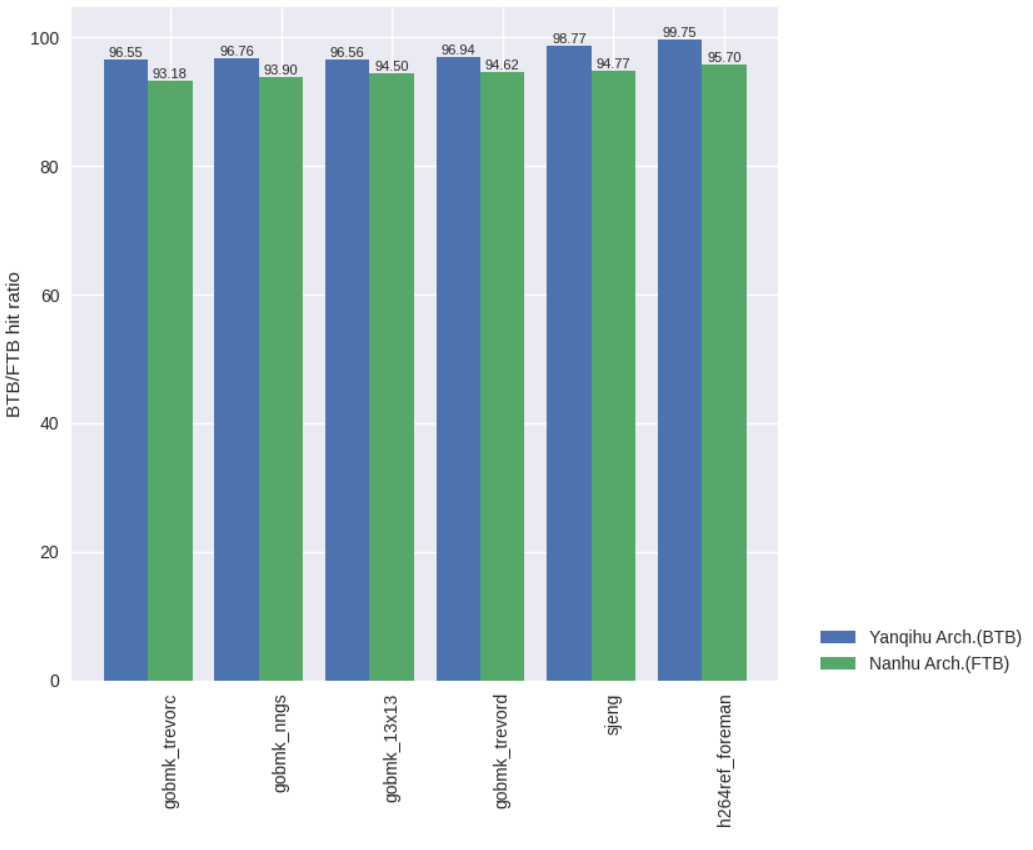
\includegraphics[width=0.9\textwidth]{ftb-hit-ratio.png}
	\caption{SPEC CPU 2006 coverage 0.8 部分检查点FTB/BTB命中率对比}
	\label{fig:figure63}
\end{figure}

% \begin{table}[]
%     \caption{两版架构频率对比}
%     \label{tb:table1}
%     \centering
%     \begin{tabular}{|c|c|c|}
%         \hline
%         版本   & 工艺   & 主频   \\ \hline
%         雁栖湖架构 & 28nm & 1.3GHz \\ \hline
%         雁栖湖架构 & 14nm & 1.8GHz \\ \hline
%         南湖架构 & 14nm & 2.0GHz \\ \hline
%     \end{tabular}
% \end{table}

频率方面是雁栖湖架构和南湖架构中前端最主要的提升。香山雁栖湖架构流片时使用的是28nm的制作工艺,主频能够达到1.3GHz,而用14nm的工艺库评估香山雁栖湖架构,最高能够达到1.8GHz的主频。香山南湖架构流片使用的是14nm工艺,主频能够达到2GHz。如表\ref{tb:table3}所示。在雁栖湖架构的基础上,通过重构分支预测部件,降低预测宽度,修改预测算法的实现等优化后,南湖架构的总体时序评估结果,在相同的14nm工艺库下,能够做到的主频相比于雁栖湖架构提升了11\%。

~\\

\begin{table}[!h]
	\caption{香山雁栖湖架构和南湖架构频率对比}
	\label{tb:table3}
	\centering
	\begin{tabular}{|c|c|c|}
		\hline
		架构版本   & 工艺库   & 主频   \\ \hline
		雁栖湖架构 & 28nm & 1.3GHz \\ \hline
		雁栖湖架构 & 14nm & 1.8GHz \\ \hline
		南湖架构 & 14nm & 2.0GHz \\ \hline
	\end{tabular}
\end{table}


\section{本章小结}

本章主要介绍了整个项目在进行测试和性能评估时使用的工具和方法,并从多个角度分析了南湖架构相比于雁栖湖架构带来的改变。这也是在频率和性能之间不断进行权衡比较的结果,相比于雁栖湖架构,南湖架构分支预测的性能有小幅的提升,而最终的总体性能,以及能够达到的最终流片频率均有较大的提升。						
% !Mode:: "TeX:UTF-8"

\chapter{总结与展望}

\section{总结}

在高性能处理器的分支预测研究领域中,为了提高分支预测准确率,大量的学者提出了各种各样的算法和改进措施,也取得了很好的效果。但是大部分论文中的算法设计都是基于模拟器进行性能分析,并没有考虑到现实物理设计时的限制,而商业处理器的分支预测具体设计大部分细节都不会公开。

而本文选用香山这一RISC-V开源高性能处理器作为平台,在其第一版雁栖湖架构的分支预测部件基础上进行了重构和改进,提出了一种新分支预测架构的设计实现,其中主要的两个改进:实现FTB相关改动以限制分支预测宽度,以及将分支预测和取指单元的流水线解耦来减少前端流水线的气泡。此外一些分支预测器中也有许多优化逻辑电路延迟的改动。最终作为香山处理器第二版南湖的分支预测组件设计,即将送往流片。南湖架构相对于雁栖湖架构来说,分支预测性能,总体性能和频率都有一定的提升。在相同的14nm工艺下,使用Design Compiler进行评估,整体的频率能够从雁栖湖架构的1.8GHz提升到2.0GHz,提升了11\%,且从SPEC 2006下的部分测试程序结果来看,整体IPC性能能够提升30.96\%。

\section{展望}

本文提出的分支预测架构在雁栖湖架构的基础上做出了改进,取得了良好的效果,但是其实目前的设计还有很多不足和待改进的地方。这里提出一部分改进思路和未来的研究方向:

\begin{enumerate}
    \item 在开发过程中,如何快速准确的对分支预测部件进行功能评估,一直是一个没有解决的问题,由于分支预测本身就是一个预测性质的功能,即使预测错误也只是会造成性能损失,不会出现功能上的错误,因此香山的差分测试框架难以找到分支预测实现上的bug。如何测试分支预测运行时各种功能是否正常,是一个非常值得深入研究的课题。
    \item 在香山下一版的设计,以及未来的每次迭代中,对频率和性能的要求肯定是越来越高的,因此在南湖架构的基础上,需要考虑如何能够做到更高的频率,如何做到更高的分支预测准确率,都是值得研究的课题。可能分支预测的整体框架还要大幅的改动。
    \item 在雁栖湖架构的设计中,分支预测里实现了循环预测器,但是在南湖架构中移除了它,主要是因为南湖架构使用了非对齐的取指策略,同一条分支可能存在于不同的Fetch Block中,这样对于循环预测器的实现带来了一些问题,循环预测器无法准确的记录某条循环跳转指令的迭代次数。因此之后如何设计实现循环预测器,将其加入到分支预测中,也是一个未来的改进方向。
\end{enumerate}




% 参考文献
% 若是要对参考文献进行重新编译,需要先使用clean.bat或是clean.sh清除辅助文件
\defaultfont
\bibliographystyle{HNUThesis}
\phantomsection
\addcontentsline{toc}{chapter}{参考文献}          	% 参考文献加入到中文目录
%\nocite{*}                                        	% 若将此命令屏蔽掉,则未引用的文献不会出现在文后的参考文献中。 
\bibliography{references}					

\renewcommand\thefigure{A.\arabic{figure}}			% 将附录中的图像的id的章节num设置为A
% \include{data/appendix}                   			% 附录
% !Mode:: "TeX:UTF-8"

\newenvironment{theacknowledgements}{\wuhao\song}

\addcontentsline{toc}{chapter}{致谢}%添加到目录中
\chapter*{\centering\xiaosan\hei\bfseries 致\quad 谢}

\begin{theacknowledgements}
	
% 随着三年硕士研究生生活的落幕,也代表着我多年的求学生活已经到达了尾声,我很庆幸在学生生涯的最后一段时间能够遇到我的导师和同学们,他们在学习和生活上给予了我许多的帮助,也很感谢深圳大学,虽然因为疫情和实习原因,我真正待在校园里的时间不长,但美丽的景色,舒适的宿舍,还有导师和同学们,都使得这三年将会成为我今后不断怀念的一段时光。

% 首先我要感谢我的导师,***老师,是他带领我踏入了计算机体系结构的领域,我在本科时学习的是软件专业,后来由于对硬件设计感兴趣而找到了*老师,*老师在三年间给了我许许多多的指导,让我从之前对计算机体系结构和硬件设计几乎零基础,到今天能够参加大型的工程项目,并积累了许多宝贵的经验。这一切都离不开*老师的指导和帮助。

% 此外还要感谢在实习期间,同样给予我许多指导的包云岗老师,唐丹老师,解壁伟老师,郇丹丹老师,赵继业老师,李祖松老师,他们让我了解了业内顶尖的学者和工程师的风貌,也传授给我许多宝贵的经验。同样感谢的还有在实习中所有的同学们,在我入门时耐心的给我解答问题,在毕业时也给了我大量的帮助。

% 还要感谢同门的毕壹双、甘海洋、罗浩鑫师兄和陈子韵师姐,张发旺,陈仕健和曾智圣同学,以及我的室友们,在平时工作中大家是可靠的伙伴,能够一起交流探讨许多有趣的问题和技术,生活中也是亲密的朋友,大家一起聊天聚餐,使科研生活增添了许多色彩。

% 最后感谢我的父母和我的亲人们,一直以来都在默默地支持着我,支持我所有的选择,无论在外有多辛苦,只要我回到家中,就能够由衷地感到一种宁静与放松。他们对我的支持也能够让我能够全身心投入到学习和工作中。

% 一个篇章的落幕是另一段新篇章的开始。我即将正式踏入社会,未来充满了未知和挑战,也有无数新的风景与人等着我去发现。抛去对未来的迷茫,我更多的是对新生活的向往与好奇。今后的路还很长,我已经准备好迎接新的挑战,无论结果如何,我都会不断努力,不辜负所有曾在我人生道路中帮助过我的人对我的期望。

\end{theacknowledgements}





						% 致谢
% !Mode:: "TeX:UTF-8"

\newenvironment{thepublications}{\wuhao\song}

\addcontentsline{toc}{chapter}{攻读硕士学位期间的研究成果}%添加到目录中
\chapter*{\centering\xiaosan\hei\bfseries 攻读硕士学位期间的研究成果}

\begin{thepublications}

\setlength{\parindent}{0em}
\begin{publist}
	% \item	\cite{my-paper}
	\item 邹江瑞, 蔡晔, Tang D, et al. A Design of Fetch Target Buffer Implemented on XiangShan Processor. In: Proc of 2022 International Conference on Computer Architecture and Software Engineering. 2022. 已录用,第一作者
	\item 蔡晔, 邹江瑞. 一种IUM的设计及其实现. 发明专利,已受理
\end{publist}

\vfill
\hangafter=1\hangindent=2em\noindent

\setlength{\parindent}{2em}

\end{thepublications}

							% 研究成果
\clearpage

\end{CJK*}                                        	% 结束中文字体使用
\end{document}                                    	% 结束全文
